% TENTH VERSION (v10): same numbers as v9; six data figures added (figures/fig_v10_*.tex, v10_*.pdf, drawn by
% ../gen_v10/make_figures.py from out/qcore{6,7,8,9}_heldout/results.json; plotted values in ../gen_v10/figdata.json),
% tab_main6 and tab_d9 moved to the appendix, and the long appendix listings moved to supplement.tex (-> ../supplement.pdf),
% cut verbatim by ../gen_v10/split_parts.py into parts/. Cross-references via xr-hyper. Previous version: ../latex2col_v9/.
% Two-column build of paper/draft_general.md (hand-maintained), ninth version (frozen qcore9 on the new real held-out SEC set 4
% = set D; frozen qcore6 on the earlier real held-out sets; frozen qcore7 and qcore8 on fresh synthetic held-out sets and the dev grids).
% tab_d9.tex and appendix_q9.tex are generated by ../gen_v9/gen_q9_tex.py from out/qcore9_heldout/results.json; ../V9_NUMBERS_CHECK.md. Every number comes from
% draft_general.md or the result files its HTML comments cite; per-figure and per-table sources are noted in figures/*.tex,
% tab_*6.tex and appendix_q6.tex (generated by ../gen_v6/gen_q6_tex.py from out/qcore6_heldout/results.json), and
% tab_q7.tex, tab_dev7.tex and appendix_q7.tex (generated by ../gen_v7/gen_q7_tex.py from out/qcore7_heldout/results.json
% and out/qcore7_work/dev_summary7.json), and tab_q8.tex, tab_dev8.tex and appendix_q8.tex (generated by ../gen_v8/gen_q8_tex.py
% from out/qcore8_heldout/results.json and out/qcore8_work/dev_report8.json). Number-by-number sources: ../V6_NUMBERS_CHECK.md,
% ../V7_NUMBERS_CHECK.md and ../V8_NUMBERS_CHECK.md.
% Previous versions: ../latex2col_v8/ (qcore8), ../latex2col_v7/ (qcore7), ../latex2col_v6/ (qcore6), ../latex2col_v5/ (qcore5), ../latex2col_v3_q4/ (qcore4), ../latex2col_v2_general/, ../latex2col_v1_pe/.
\documentclass[10pt,twocolumn]{article}
\usepackage[letterpaper,margin=0.75in,columnsep=0.25in]{geometry}
\usepackage[T1]{fontenc}
\usepackage{mathptmx}
\usepackage[scaled=0.9]{helvet}
\usepackage{courier}
\usepackage{microtype}
\usepackage{amsmath,amssymb}
\usepackage[numbers,sort&compress]{natbib}
\usepackage{booktabs,tabularx,array,multirow}
\usepackage{graphicx}
\graphicspath{{figures/}{latex2col/figures/}}
\usepackage{xcolor}
\usepackage{pifont}
\usepackage{tikz}
\usetikzlibrary{arrows.meta,positioning,patterns,calc}
\usepackage{pgfplots}
\pgfplotsset{compat=1.18}
\usepgfplotslibrary{groupplots}
\usepackage[font=small,labelfont=bf,skip=4pt]{caption}
\usepackage{enumitem}
\usepackage{needspace}
\usepackage{adjustbox}
\usepackage{longtable}
\setlist{nosep,leftmargin=1.2em}
\usepackage{xr-hyper}
\externaldocument[]{supplement}
\usepackage[colorlinks=true,linkcolor=blue!45!black,citecolor=blue!45!black,urlcolor=blue!45!black]{hyperref}
\usepackage{xurl}

% ---- one palette for every chart and diagram (validated with the dataviz checker) ----
\definecolor{cFix}{HTML}{2A78D6}    % fixed by tier 1
\definecolor{cT2}{HTML}{EDA100}     % sent to tier 2 / flagged
\definecolor{cMiss}{HTML}{C9C7C0}   % missed (neutral, hatched for grayscale)
\definecolor{cWrong}{HTML}{E34948}  % wrong change / silent wrong
\definecolor{ink}{HTML}{52514E}     % secondary text, axes

\pgfplotsset{
  qbar/.style={xbar stacked, bar width=7pt, scale only axis,
    axis line style={draw=ink!60}, tick style={draw=ink!60},
    axis x line*=bottom, axis y line*=left, y axis line style={draw=none}, ytick style={draw=none},
    tick label style={font=\sffamily\scriptsize, text=black},
    label style={font=\sffamily\scriptsize, text=ink},
    title style={font=\sffamily\scriptsize\bfseries, yshift=-3pt},
    xmajorgrids, grid style={draw=ink!15},
    enlarge y limits={abs=0.55},
    legend style={font=\sffamily\scriptsize, draw=none, fill=none, column sep=6pt},
    legend image code/.code={\draw[#1] (0cm,-0.09cm) rectangle (0.32cm,0.09cm);},
  },
  gbar/.style={xbar, bar width=4.6pt, scale only axis,
    axis line style={draw=ink!60}, tick style={draw=ink!60},
    axis x line*=bottom, axis y line*=left, y axis line style={draw=none}, ytick style={draw=none},
    tick label style={font=\sffamily\scriptsize, text=black},
    label style={font=\sffamily\scriptsize, text=ink},
    title style={font=\sffamily\scriptsize\bfseries, yshift=-2pt},
    xmajorgrids, grid style={draw=ink!15},
    enlarge y limits={abs=0.62}, clip=false,
    point meta=explicit symbolic,
    nodes near coords, nodes near coords align={horizontal},
    every node near coord/.append style={font=\sffamily\tiny, text=black, inner sep=1.5pt, anchor=west, rotate=0},
    legend style={font=\sffamily\scriptsize, draw=none, fill=none, column sep=5pt},
    legend image code/.code={\draw[#1] (0cm,-0.09cm) rectangle (0.32cm,0.09cm);},
  },
  silentbar/.style={fill=cWrong, draw=white, line width=0.4pt},
  flagbar/.style={fill=cT2, draw=white, line width=0.4pt},
  brokebar/.style={fill=cMiss, draw=ink!60, line width=0.4pt,
    postaction={pattern=north east lines, pattern color=ink!55}},
  fixbar/.style={fill=cFix, draw=white, line width=0.6pt},
  t2bar/.style={fill=cT2, draw=white, line width=0.6pt},
  missbar/.style={fill=cMiss, draw=white, line width=0.6pt,
    postaction={pattern=north east lines, pattern color=ink!55}},
  dotplot/.style={scale only axis,
    axis line style={draw=ink!60}, tick style={draw=ink!60},
    axis x line*=bottom, axis y line*=left, y axis line style={draw=none}, ytick style={draw=none},
    tick label style={font=\sffamily\scriptsize, text=black},
    title style={font=\sffamily\scriptsize\bfseries, yshift=-3pt},
    xmajorgrids, grid style={draw=ink!15}, enlarge y limits={abs=0.5}, clip=false},
  dotmark/.style={only marks, mark=*, mark size=2.2pt, color=cFix!85!black,
    mark options={draw=white, line width=0.5pt},
    error bars/error bar style={line width=0.8pt, color=cFix!85!black},
    error bars/error mark options={rotate=90, mark size=2pt, line width=0.8pt}},
}
\tikzset{
  inlab/.style={font=\sffamily\scriptsize\bfseries, text=white},
  darklab/.style={font=\sffamily\scriptsize, text=black},
  sidelab/.style={font=\sffamily\tiny, text=ink, anchor=west, xshift=2pt},
  misslab/.style={font=\sffamily\scriptsize, text=black, fill=cMiss, inner sep=1pt, rounded corners=1pt},
  wronglab/.style={font=\sffamily\scriptsize, text=black, anchor=west, xshift=2pt},
  vlab/.style={font=\sffamily\tiny, text=ink, above=3.5pt},
}

\raggedbottom
\newcommand{\vq}[1]{\textsf{qcore#1}}
\newcommand{\code}[1]{\texttt{\small #1}}
\newcommand{\Fail}{\mathcal{F}}
\newcommand{\Tie}{\mathcal{T}}
\renewcommand{\topfraction}{0.9}
\renewcommand{\dbltopfraction}{0.9}
\renewcommand{\textfraction}{0.1}
\renewcommand{\floatpagefraction}{0.8}
\renewcommand{\dblfloatpagefraction}{0.8}
\setlength{\textfloatsep}{10pt plus 2pt minus 2pt}
\setlength{\dbltextfloatsep}{10pt plus 2pt minus 2pt}
\setlength{\abovedisplayskip}{4pt plus 1pt minus 1pt}
\setlength{\belowdisplayskip}{4pt plus 1pt minus 1pt}
\setlength{\bibsep}{1.5pt}
\newcolumntype{L}{>{\raggedright\arraybackslash}X}
\newcommand{\tsize}{\footnotesize\setlength{\tabcolsep}{3.5pt}}


\title{\Large\bfseries A Cheap Model and a Deterministic Checker: Fewer Silent Errors in Numeric Document Extraction from the Documents' Own Identities}
\author{Aarush Yadav\\\texttt{ayadav361@ucla.edu}\and Arihan Yadav\\\texttt{apyadav@wisc.edu}}
\date{}

\begin{document}
\twocolumn[{%
\maketitle
\vspace{-2.2em}
\begin{center}
\begin{minipage}{0.86\textwidth}
\small
\noindent\textbf{Abstract.}
Investors, customers and limited partners of asset managers, private equity and venture capital firms, and alternative market data providers receive a steady stream of financial statements, from quarterly packets for each private fund to the 10-Qs and 10-Ks of public companies, and cheap vision-language models are increasingly used to extract the numbers. Those numbers are usually right; the costly ones are wrong and unflagged, which we call \emph{silent}. Many document sets constrain their own numbers through linear identities $Ax=b$: totals, roll-forwards, quantity times price, the same figure printed twice. We put a deterministic checker between a cheap model and a stronger model or a person. It changes a value only when an identity, or an unambiguous and corroborated read of the printed page, backs the change, and it sends every other doubt on with its evidence. Nothing in it names a domain, and it can discover its identities from the page with no configuration. Each version is tuned on development data, frozen and run once on held-out data. The latest, \vq{9} (first freeze, sha256 \code{3ca510d3\dots}), was run once on 24 SEC filings locked before its freeze (72 statements, 5,351 numbers, 16 10-Qs and 8 10-Ks), read from poor scans that keep a born-digital text layer. There Claude Haiku with the checker leaves 9 silent errors (95\% CI 0--26) where Claude Opus alone leaves 25; on this set alone the paired difference, $-16$ ($-43$ to $+10$), is not significant, because Opus made few errors. On the 22 filings of the previous real test it was 15 against 50 ($-35$, $-73$ to $-6$), and pooled over four held-out SEC sets (227 statements, 17,125 numbers) it is 28 against 174 ($-146$, $-231$ to $-72$; 32 if the earlier version is used on all four). On the new filings Opus with the checker leaves no silent error and GPT goes from 1,090 to 15. In the first real held-out test of the final zero-config mode, with no identity or schema file, Haiku leaves 16 silent errors and GPT 37 (\vq{8}: 51), more than with hand-written identities (9 and 15); every zero-config run with the text layer broke the same three numbers, cash-flow totals whose closing parenthesis the filing's text layer prints as a separate word. On synthetic held-out sets zero-config left 2 to 7 times the silent errors of hand identities. A re-read of unsure cells by a vision model is not independent evidence: its errors are correlated with the extraction's; the identities' are not. Without a trustworthy text layer the cheap model does not overtake the strong one.
\end{minipage}
\end{center}
\vspace{1.2em}
}]

% Figure 1 (v6): the tier ladder. Counts: Claude Haiku on the 155 held-out SEC statements (sets 1-3 pooled),
% poor scans, frozen qcore6, hand identities, text mode (out/qcore6_heldout/results.json, sets.ABC.rows
% "Haiku + qcore6 (text)": 527 tier 0 errors (Haiku alone wrong); fixed 348; wrong at the end 179, flagged wrong 160,
% silent 19; broken 0; tier 2 items 25 (A) + 55 (B) + 75 (C) = 155 (sets.{A,B,C}.rows[...].tier2_items).
\begin{figure*}[t]
\centering
\def\hdr{\small\bfseries}
\begin{tikzpicture}[
  font=\sffamily\footnotesize,
  tier/.style={draw=ink, rounded corners=2pt, line width=0.6pt, fill=white, align=left,
               inner sep=4pt, text width=#1, minimum height=2.75cm,
               execute at begin node={\hyphenpenalty=10000\exhyphenpenalty=10000}},
  tier/.default=3.0cm,
  hdr/.style={font=\sffamily\small\bfseries},
  flow/.style={-{Latex[length=2.2mm,width=1.6mm]}, line width=0.8pt, draw=ink},
  lab/.style={font=\sffamily\scriptsize, text=ink, align=center, text width=1.55cm},
  stage/.style={draw=cFix!70!black, fill=cFix!8, rounded corners=1.5pt, inner sep=2pt,
                text width=3.45cm, align=left, font=\sffamily\scriptsize, minimum height=0.40cm},
  opt/.style={draw=cT2!80!black, fill=cT2!10, dashed, rounded corners=1.5pt, inner sep=2pt,
                text width=3.45cm, align=left, font=\sffamily\scriptsize, minimum height=0.40cm},
]
% Tier 0
\node[tier=2.25cm] (t0) at (0,0) {%
  {\hdr Tier 0}\\[1pt] cheap model\\[1pt]
  {\scriptsize\color{ink} any extractor reading page images (here Haiku)}\\[3pt]
  {\scriptsize every document}};
% Tier 1 container
\node[draw=cFix!80!black, line width=0.9pt, rounded corners=2pt, fill=cFix!3,
      minimum width=4.5cm, minimum height=4.35cm] (t1) at (5.05,-0.40) {};
\node[hdr, anchor=north west] at ([xshift=3pt,yshift=-2pt]t1.north west) {Tier 1 \textmd{deterministic checker}};
\node[stage, anchor=north] (s1) at ([yshift=-0.50cm]t1.north) {\textbf{a} identities $Ax=b$: hand-written, discovered on the page, or both};
\node[stage, below=1.5pt of s1] (s2) {\textbf{b} label read, gated and guarded (OCR: second reader)};
\node[stage, below=1.5pt of s2] (s3) {\textbf{c} repair search (swap, period, sign) and misread repair};
\node[stage, below=1.5pt of s3] (s4) {\textbf{d} route the rest with evidence};
\node[opt, below=1.5pt of s4] (s5) {\textbf{e} optional re-read of unsure cells: flags; a value moves only if an identity ties};
% Tier 2
\node[tier=2.55cm] (t2) at (10.3,0) {%
  {\hdr Tier 2}\\[1pt] stronger model\\[1pt]
  {\scriptsize\color{ink} answer checked by the same rules}\\[3pt]
  {\scriptsize only what tier 1 does not settle}};
% Tier 3
\node[tier=2.25cm] (t3) at (14.75,0) {%
  {\hdr Tier 3}\\[1pt] a person\\[3pt]
  {\scriptsize\color{ink} only what tier 2 cannot settle, or a fix that fails the check}};
\node[lab, anchor=south, text width=2.6cm] (pdf) at ([yshift=10pt]t0.north) {any PDF set whose numbers obey linear identities};
\draw[flow] (pdf.south) -- (t0.north);
\draw[flow] (t0.east) -- node[lab, above=1pt] {records} node[lab, below=1pt] {key, value,\\page, printed\\text} (t1.west |- t0.east);
\draw[flow] (t1.east |- t2.west) -- node[lab, above=1pt] {packets} node[lab, below=1pt] {160 errors\\in 155 items} (t2.west);
\draw[flow] (t2.east) -- node[lab, above=1pt] {alerts} node[lab, below=1pt] {unsure, document\\error, failed\\check} (t3.west);
\node[lab, anchor=north, text width=4.6cm, fill=cFix!12, draw=cFix!80!black, rounded corners=1.5pt, inner sep=3pt]
  (fix) at ([yshift=-9pt]t1.south) {\textbf{fixed values} (corrections log)\\
  \textbf{348 of 527 errors (66\%)}; 0 broken, 19 silent};
\draw[flow] (t1.south) -- (fix.north);
\node[font=\sffamily\scriptsize, text=ink, anchor=north, inner sep=2pt] (vfix) at ([yshift=-9pt]t2.south) {checked fix $\rightarrow$ correction};
\draw[flow] (t2.south) -- (vfix.north);
\end{tikzpicture}
\caption{The tier ladder. A cheap model extracts; a deterministic checker writes a value only when the page and the documents' own linear identities agree, and sends everything else on as small packets with evidence; a stronger model or a person sees only those. Nothing in tier~1 names a domain. Counts: Claude Haiku on the 155 held-out SEC statements read from poor scans (11,774 numbers; frozen \vq{6}, hand identities, born-digital text layer).}
\label{fig:ladder}
\end{figure*}


% =====================================================================
\section{Introduction}

Investors, customers and limited partners of asset managers, private equity and venture capital firms, and alternative market data providers receive a steady stream of financial statements: a quarterly packet of statements from each private fund, and the quarterly and annual filings of every public company they follow. Cheap vision-language models are increasingly used to extract the numbers, and the numbers feed valuations, investor reports and trades. These documents, like many others, are internally redundant. A balance sheet prints its totals; a cash-flow statement rolls a balance forward; an invoice prints line amounts, a subtotal, tax and a total; a receipt prints quantity, unit price and amount; a statistical bulletin prints rows and the column that adds them. Write the extracted values as a vector $x$: the document set asserts $Ax=b$ up to rounding. This paper is about using that redundancy, and the printed page, to catch the errors a model makes without telling anyone.

On clean pages the strongest models rarely err. On 21,367 numbers in clean SEC notes tables Claude Opus made no error, and on 7,892 numbers of synthetic reports, invoices and bulletins it made none either (Section~\ref{sec:safety}). Reading is not always easy: a pipeline rasterises a filing at low resolution, a statement arrives as a fax, a receipt as a phone photo. On poor scans of 227 held-out SEC statements Opus is 98.98\% accurate, Claude Haiku 95.94\% and GPT 76.20\%. A wrong number that some check points at costs a reviewer a minute; one that nothing points at goes into a model, a filing or a payment. We count those \emph{silent} errors. Strong models' errors can be harder to catch, partly because the models say that when a digit is unclear they pick the value that makes the totals add up (Section~\ref{sec:bend}). Any check that only sums the extraction accepts that number.

We describe a ladder (Figure~\ref{fig:ladder}). A cheap model extracts. A deterministic checker, which uses no model, reads the page, tests the identities, and writes a value only when an identity backs the change or the read of that exact cell is unambiguous and corroborated; it may write only a number the field's own line prints or one already extracted. Everything else goes up as a small packet with its evidence, to a stronger model or a person. The method needs no domain code: the identities and field labels are inputs, and the sixth to ninth versions discover them from the documents themselves when none are given. Our findings:
\begin{enumerate}
\item \textbf{Replication on new filings, twice.} On 22 filings built after \vq{6} was frozen, Haiku plus the checker leaves 15 silent errors against Opus alone's 50 ($-35$, $-73$ to $-6$). On 24 further filings locked before \vq{9} was frozen it leaves 9 against 25: fewer, but not significantly ($-16$, $-43$ to $+10$), as Opus alone erred little there. Pooled over four SEC sets it is 28 against 174 ($-146$, $-231$ to $-72$) (Section~\ref{sec:headline}).
\item \textbf{It helps every model.} Opus, Haiku and GPT, eight held-out sets: significant cuts in 50 of 60 per-set settings with \vq{6} and 11 of 12 with \vq{9} on the newest filings, where Opus's silent errors fall from 25 to 0 and GPT's from 1,090 to 15. Every broken number is listed with its cause (Section~\ref{sec:allmodels}).
\item \textbf{Zero configuration works, but less well.} On the newest filings, with no identity or schema file, the checker leaves Haiku 16 silent errors and GPT 37, against 9 and 15 with hand-written identities and 168 and 1,090 for the models alone; it breaks three correct numbers per model where a text layer misprints signs. On synthetic held-out sets it leaves 2 to 7 times the silent errors of hand identities, mostly on layouts it was never tuned on (Sections~\ref{sec:zeroconfig} and~\ref{sec:q7}).
\item \textbf{A second read is not independent evidence.} A vision-model re-read of unsure cells repeats the extraction's wrong digit often enough (32\% of wrong cells for a Haiku reader, 16\% for Opus, on development data) that we let it move a value only through an identity. Held out, it changed nothing and made a few errors visible (Section~\ref{sec:reread}).
\item \textbf{Where it stops.} Without a born-digital text layer the cheap model does not catch up, on any SEC set, though the checker still cuts the strong model's silent errors (Section~\ref{sec:ocr}).
\end{enumerate}
We claim no novelty for the repair operations (Section~\ref{sec:related}). What we add is the page-grounded gate, identity discovery validated on the page, a measured account of model-on-model re-reading, and an evaluation protocol that freezes code before every held-out run.

% =====================================================================
\section{Related work}\label{sec:related}

Correcting sign errors, swapped values and typing errors under linear balance edits is established in official statistics and is the direct prior art for our repair step. Scholtus finds a minimal set of sign flips and swaps that makes a record consistent, and accepts a rounding repair only if it creates no new edit violations~\citep{scholtus2011algorithms}; an earlier report corrects single-digit typing errors~\citep{scholtus2009typing}. The deducorrect package implements typo, sign and swap correction and touches no variable in a satisfied edit~\citep{vanderloo2011deducorrect}; its acceptance rule is ours. The deductive, automatic, then manual editing process~\citep{pannekoek2013automated} has the shape of our tiers, and error localisation goes back to Fellegi and Holt~\citep{fellegi1976systematic}. DART repaired OCR'd balance sheets under aggregate constraints with an operator accepting each update~\citep{fazzinga2006dart,flesca2010querying,bertossi2005complexity}; an IPUMS tool locates OCR digit errors in census tables from row and column totals~\citep{kugler2026ipums}; Correia and Luck flag OCR'd balance sheets with accounting identities~\citep{correia2023digitizing}. These impute any value that satisfies the constraints, or only flag; ours admits only values the page prints on the field's own line or that were already extracted.

Hemmer et al.\ filter LLM extractions of CORD and SROIE receipts with arithmetic constraints~\citep{hemmer2025neurosymbolic}, and Aggarwal et al.\ flag failing sums in fiscal documents~\citep{aggarwal2025fiscal}. Financial verification systems check claims or detect inconsistencies in statements and XBRL~\citep{hall2026verifin,panda2026finverbench,wang2026auditflow,wang2025finauditing,shu2025lava}; none repairs extracted values against the page. Totals in early XBRL filings often did not equal their components~\citep{debreceny2010add}, one reason not to take filed identities on trust. We use CORD~\citep{park2019cord}, Donut~\citep{kim2022donut} and the VRDU ad-buy forms~\citep{wang2023vrdu}. VLMs invent characters on degraded documents~\citep{he2025seeing}, and OCR noise corrupts numbers in LLM key-value extraction~\citep{anvari2026pixels}. Model cascades route on learned scores, self-verification or confidence~\citep{chen2024frugalgpt,aggarwal2024automix,shankar2026taskcascades,gupta2024cascades,jung2025trust}; our gate is a deterministic identity test plus page evidence. LLMs do not reliably self-correct without external feedback~\citep{huang2024cannot}, and models satisfy a visible check rather than the intended goal~\citep{zhong2025impossiblebench,baker2025monitoring}; our re-read results add that a second model read of the same pixels is correlated with the first.

% =====================================================================
\section{Method}\label{sec:method}

\subsection{Inputs and identities}
A \emph{bundle} is a set of PDFs, optionally with a schema and a list of identities (truth is used only for scoring). The schema gives each field's printed labels, units and sign convention. A record's key is its document, field, period, entity (a row-group heading such as a segment or a receipt item) and column. An extraction is a list of key, value, page and printed text; a missing key is a blank. Domain knowledge lives only in the schema, the identities and a small adapter per data source; the core names no field, document or dataset.

Identity $k$ has a coefficient row $a_k$ on inputs $I_k$, a constant $b_k$ and a tolerance $\tau_k$ (half a printed rounding unit per term):
\begin{equation}\label{eq:check}
g_k(x) = a_k^{\top}x - b_k, \qquad \text{$k$ ties} \iff |g_k(x)| \le \tau_k .
\end{equation}
Product terms (count times unit price) are allowed; search and repair then use the partial derivative as the coefficient. An identity with a blank input is skipped, not failed. $\Fail(x)$ and $\Tie(x)$ are the failing and tying identities. In our data the identities are a 10-Q filer's XBRL calculation linkbase plus the balance-sheet equation and cash roll-forward; receipt arithmetic; bulletin row and column sums; a fund's roll-forwards and accumulation across quarters; or, in zero-config mode, whatever Section~\ref{sec:discover} finds.

\subsection{Label read, gate and guard}\label{sec:labelread}
Before any arithmetic the checker reads the page. For each record it finds the field's \emph{own line}, the line whose words best match a label, and the column from the header cell above; if no number or two numbers sit under that header, the read is empty. A unit statement (``in thousands'') sets a scale $s$, and a printed $p$ matches $v$ when $|p\,s-v|\le s/2$. If the printed $p_i\neq x_i$, the read proposes $x_i\leftarrow p_i$.

A proposal passes the \emph{gate} only under one of two rules. (a) \emph{Identity-backed}: it makes an identity through the cell tie that did not, and breaks none that tied. (b) \emph{Unambiguous and corroborated}: the label matches exactly one line in the document, the header places the cell, no other column lands on it, and the extraction corroborates the read (a sign flip, a one-glyph misread, a blank filled, or the extracted number printed elsewhere on the row or nowhere in the document). A read never changes a value by a power of 1000. Passing reads are applied jointly under a \emph{guard}: a tied identity may break only if every read feeding it is backed by its field's single best line. Every other read becomes a tier~2 item with its reason.

\subsection{Repair search and routing}
For each failing identity and input $i$, the search tries swapping $x_i$ with another number of the document, with the same line in the adjacent period, and negating it. A candidate $x'$ counts only if
\begin{equation}\label{eq:accept}
\Fail(x')\subsetneq\Fail(x)
\end{equation}
and the page does not contradict it. A closing value $v=x_i-g_k(x)/a_{ki}$ is kept only if every failing identity through $i$ implies it, it is a digit-level misread of $x_i$, \eqref{eq:accept} holds and $v$ is printed on $i$'s own line. So every value the checker writes lies in
\begin{equation}\label{eq:allowed}
x'_i \in \{p_i\}\ \cup\ \{x_j,\,-x_j : j \text{ extracted}\}:
\end{equation}
it never invents a number to make the books tie. Remaining failures become tier~2 items naming only the inputs not shown to be right; when every input matches the page, the item is a source-document error and the values stay. Without page text the checker writes nothing except a flip back to a declared sign.
Figure~\ref{fig:algo} summarises the steps.

\begin{figure}[t]
\centering
\fbox{\begin{minipage}{0.94\columnwidth}\small
\textbf{Checker} (one document; extraction $x$, identities $Ax=b$, page reads $p$)\\[2pt]
\begin{tabular}{@{}r@{\hspace{5pt}}p{0.86\columnwidth}@{}}
1: & Label each read: \emph{corroborated} if $x_i$ matches the page on $i$'s own line.\\
2: & $\Fail(x)\gets\{k : |g_k(x)|>\tau_k\}$, where $g_k(x)=a_k^\top x-b_k$.\\
3: & \textbf{for} each $k\in\Fail(x)$ and input $i$ of $k$ \textbf{do}\\
4: & \quad candidates $x'$: swap $x_i$ with another number, with the adjacent period's value, or negate it; or the closing value $v=x_i-g_k(x)/a_{ki}$.\\
5: & \quad \textbf{keep} $x'$ only if $\Fail(x')\subsetneq\Fail(x)$ \eqref{eq:accept}, the page does not contradict it, and $x'_i$ lies in the allowed set \eqref{eq:allowed}.\\
6: & \quad \textbf{gate:} write $x'$ only if (a) it is backed by an identity or (b) the read is unambiguous and corroborated.\\
7: & \textbf{for} each $k$ still in $\Fail$ \textbf{do}\\
8: & \quad \textbf{if} every input of $k$ matches the page: mark a source-document error; keep values.\\
9: & \quad \textbf{else} route to tier~2, naming only inputs not shown right.\\
10: & \textbf{return} $x$, tier-2 items.
\end{tabular}
\end{minipage}}
\caption{The checker's decision steps. It never writes a value outside the allowed set, so it cannot invent a number to make the books tie.}
\label{fig:algo}
\end{figure}


\subsection{What the checker reads}\label{sec:textmode}
\emph{Text mode} reads the PDF's text layer while the model reads a page image: a born-digital PDF that a pipeline rasterises (for CORD, the dataset's OCR annotation drawn as invisible text). \emph{No-text mode} runs the identities alone. \emph{OCR mode} is for scans: the OCR (docTR or Tesseract; for the real scans, the dataset's OCR or the scanner's layer) is a second, noisy reader. Where it agrees with the model the cell is never changed; where they disagree, the candidates are the OCR read, its one-glyph look-alikes and digit-wise mixes, and a change set is taken only if it is the unique best one under the identities. New in \vq{6}: a PDF whose page is covered by an image is a scan, and its text layer is treated as an OCR, not as the page; a read there is corroborated only by its digits. On development scans \vq{5} broke 4 correct numbers per model in text mode this way and \vq{6} breaks none.

\subsection{Zero-config: identities and schema discovered on the page}\label{sec:discover}
With \code{--identities auto} and \code{--schema auto} the bundle holds only the PDFs. Each document's records are laid out as a grid in page reading order, and candidate identities are generated as templates: \emph{row sums} (subtotals, totals and roll-forwards: spans of up to 25 rows above a row, every sign pattern up to four terms, collapsed so that a total over subtotals is found after them), \emph{column sums} (segments adding to a consolidated column), \emph{products} (quantity times price equals amount) and \emph{equal ties} across tables and documents (the same number at least 100 rounding units, same period, same duration and years in the headings, a shared label word). A template is checked on every instance, reading each cell from the page where it can and from the extraction otherwise; it is admitted if it holds on at least two instances and fails on at most $\max(1,10\%)$, and refused if the page reads it whole somewhere and never confirms it, so an identity is never invented from the extraction where the page disagrees. Field labels come from the extraction's printed text and are kept only if a page line with every word of the label prints the field's number; units and sign conventions are inferred the same way. On development data 99.7\% of the identities discovered in text mode held on the true values (12,401 of 12,437) and 99.1\% without (7,093 of 7,154). \code{--identities both} adds the discovered identities to a hand-written file.

\textbf{\vq{7} and \vq{8}.} Both change only what runs when something is discovered (\code{auto} or \code{both} identities, or \code{auto} schema) and add no new way to change a value. \vq{7} keeps label cells from being read as values (age bands, years, numbers inside a label), requires a tier~1 change resting only on discovered identities to have independent backing (a hand identity, two discovered identities that do not share most of their inputs, or one confirmed on the page in two places), adds aggregate ties, and lets the inferred schema accept \emph{weak} labels that change a value only through an identity or as a one- or two-glyph misread. \vq{8} admits more templates: a sum of four or more terms is admitted when it holds with large numbers in at least two places and fails no more often than it holds, and the page must confirm it four times as often as it refutes it where it reads every cell; it adds transposed templates, roll-forwards over the previous column, sparse sums, closing balances carried to the next statement, year-to-date accumulation and products with a rate; it sets a tolerance from the finest rounding unit two numbers show; and a weak label changes a value only through an identity. Details: Appendix~\ref{app:changes} and Supplement~\ref{sup:changes}.

\textbf{\vq{9}, the version tested on set~4.} Five generic changes, made on development data (Appendix~\ref{app:changes}, Supplement~\ref{sup:changes}); again no new way to change a value. (1) A sign proposal from the label read is dropped when the extraction's own citation is another print of the same number showing the extracted sign (a bank statement prints each check as $(542.03)$ in one list and $542.03$ in another). (2) When a candidate line spells every identifier of a record in its label (`ANA-128'), the other candidate lines are dropped. (3) A printed number matches a stored value at the page's scale only within half of the printed number's own last digit, not within half a page unit, and a percentage never does: `0.4' on a page in thousands had matched any value from $-100$ to 900. (4) A record with an entity owns only the lines that name the entity. (5) Without page text, discovery admits a plain sum whose every failure is one slip of one cell, checks long sums of large numbers that foot exactly elsewhere to 1.5 units, tries a total as the sum of the section totals above it and admits equal ties between non-adjacent totals; and a page read that rule (b) takes on its own keeps its page basis when the only identity through it is discovered. Changes 1, 2, 4 and 5 run only in zero-config code. Change 3 runs in every mode that reads the page, so with hand identities \vq{9}, unlike \vq{7} and \vq{8}, does not always return \vq{6}'s values (Section~\ref{sec:headline}).

\subsection{Re-read tier and its change gate}\label{sec:rereadmethod}
For the cells of tier~2 items (failing identities, misreads, reader disagreements, identities that tie while the OCR disagrees on a cell, blanks; at most 0.6 requests per number) the checker cuts a crop: the column header strip stitched above the cell's row, the cell outlined, deskewed and scaled. A row check moves or drops crops whose row does not print the record's label. One question asks a vision model for the printed string, the row label and the column heading; an answer naming another row or year is no evidence. The answer is a third reader of that cell, and the gate stays: a re-read may move a value only when it agrees with the page read of that exact cell \emph{and an identity through the cell then ties} (rule a). A re-read agreeing with the extraction clears a flag only when the page read is a different number altogether, not a glyph or two away. A disagreeing re-read becomes a tier~2 item with every read attached. We set this gate on development data after real reads showed why (Section~\ref{sec:reread}).

% =====================================================================
\section{Evaluation protocol and data}\label{sec:protocol}

\subsection{Freeze, tune on development data, test once}
Every version was frozen (sha256 of every file in a manifest), tuned on development data with generic fixes only, frozen again and run once on held-out data; problems found there are reported, not fixed (Table~\ref{tab:versions}). \vq{6} (28 files, combined sha256 {\small\nolinkurl{86debea05f95a6d2d93a7add48d32cd54e6109135052df4c1dd178c48a95ab34}}, frozen 2026-10-16T13:14Z, 56 tests) was tuned on development splits only; its change log lists the held-out data it did not open. The hash matched before the runs, at their end and at report time; 442 runs (\vq{6} 338, frozen \vq{5} re-run 104) each ran once, with no crash. With the hand-written identities \vq{6} returned exactly \vq{5}'s fixes and tier~2 items in all 104 (set, model, mode) runs, so the hand-identity results below are also a test of \vq{5}'s frozen rule set; \vq{6}'s new held-out evidence is the discovered identities and the re-read tier. SEC set~1 was seen before \vq{4} and \vq{5} were designed; SEC sets 2 and 3, the notes tables, the real scans and the synthetic bundles 02--05 are clean tests, and set~3 was built after \vq{5} was frozen.

\vq{7} (28 files, sha256 \code{51d9a352\dots}, frozen 2026-10-16T16:40Z, 65 tests) and \vq{8} (29 files, \code{40518616\dots}, 21:54Z, 71 tests) were tuned on every set above, all spent by then, and each was run once on a fresh synthetic set locked by a hash manifest before any of its changes (432 and 1,296 runs, no crash). \vq{8} was frozen three times before its run, each time after a development break. With hand identities \vq{7} and \vq{8} returned exactly \vq{6}'s fixes and tier~2 items in every held-out and development run.

\vq{9} (30 files, combined sha256 {\small\nolinkurl{3ca510d3ea178550ee3a43676d9f8e74a4e4ec0c4e4e8b7d4149d72732d387e0}}, frozen 2026-10-18T18:27Z, 79 tests) was tuned on every set above, \vq{8}'s fresh set included. This first freeze is the version run on set~4 and the one every \vq{9} result here describes. Its held-out test is SEC set~4. The set was built and locked (bundles 15:44Z) and its Haiku and Opus extractions (15:54Z) and GPT extractions (16:12Z) were locked by hash manifests before the freeze; \vq{9}'s change log records that neither the filings nor the set were opened while it was written. Frozen \vq{9}, \vq{8} and \vq{6} were run once on it (90 runs, 18:40--19:19Z, no crash, none repeated), with the three package hashes and the four lock manifests verified before and after. The scripts were written before any result was seen, and the modes, identity settings and scoring are set~3's. The re-read tier was not run on set~4: it needs an Opus reader answering crop requests, which that session could not run. \emph{A later refreeze.} The first freeze's development grid, run alongside, broke one new number (CAT's net income to common holders, 6,142 to 6,141\,M, in discovered-identity text runs on SEC development filings), and \vq{9} was refrozen at 19:59Z (freeze~2, \code{c4401b94\dots}) with one change in discovery (a one-unit difference no longer counts as a one-digit slip). Its freeze record still lists both freezes as before any held-out run, but by the time stamps the second came 40 minutes after the set-4 run had ended (19:19Z); a note added to the record says freeze~2 was made from the first freeze's development grid only, without seeing held-out results. Freeze~2 has not been run on set~4 or any held-out data; every \vq{9} result here is freeze~1's. Its code is kept as \code{qcore9\_f1/} (package name \code{qcore9}, since \code{qcore9/} now holds freeze~2), rebuilt by reverting the post-freeze edits; copied to a folder named \code{qcore9} it hashes to \code{3ca510d3\dots}\ exactly and its 79 tests pass.

\begin{table}[t]
\centering\tsize
\caption{Frozen versions, what each was tuned on, and what it was run on once. Earlier versions are in Appendix~\ref{app:changes}.}
\label{tab:versions}
\begin{tabularx}{\columnwidth}{@{}>{\raggedright\arraybackslash}p{0.9cm}>{\raggedright\arraybackslash}p{0.95cm}LL@{}}
\toprule
Version & Frozen (Oct.\ 2026) & Tuned on & Tested once on \\
\midrule
\vq{4} & 15th 18:33 & SEC dev filings: poor scans, OCR, injected errors; CORD train, val. & SEC 1, 2; CORD; notes; real scans \\
\vq{5} & 16th 03:28 & + notes tables of the 10 dev filers; synthetic dev; PE validation & the same, all modes, three models \\
\vq{6} & 16th 13:14 & + real-scan dev split; real re-reads of dev crops (Haiku, Opus readers) & SEC 1, 2, 3 (new); CORD; notes; real scans; synthetic 02--05 \\
\vq{7} & 16th 16:40 & + every \vq{6} held-out set (now spent); zero-config only & fresh synthetic 06--08, injected errors \\
\vq{8} & 16th 21:54 (3rd freeze) & + \vq{7}'s fresh set (now spent); zero-config only & 4 new document families; old generators 09--10; injected errors \\
\vq{9} & 18th 18:27 (1st freeze) & + \vq{8}'s fresh set (now spent); zero-config, and scaled page matches in every mode & SEC 4 (new): 24 filings, with \vq{8}, \vq{6} \\
\bottomrule
\end{tabularx}
\end{table}

\subsection{Data and models}
\textbf{SEC statements, poor scans.} Balance sheet, income statement and cash-flow statement of held-out filings: \emph{set~1}, 10 filers' 10-Qs (29 statements, 2,144 numbers); \emph{set~2}, 20 other filers' 10-Qs (60, 4,424); \emph{set~3}, 22 further filers across utilities, energy, materials, industrials, consumer, health care and financials, 15 10-Qs and 7 10-Ks (66 statements, 5,206 numbers, 1,902 of them from 10-Ks); \emph{set~4}, new for \vq{9} (\emph{set D} in the result files), 24 further filers, 16 10-Qs and 8 10-Ks (72 statements, 5,351 numbers, 1,928 from 10-Ks), built exactly as set~3. Truth is each filing's XBRL instance located on the page; identities come from the filers' calculation linkbases (set~3: 640 of 1,076; set~4: 998 of 1,135) plus semantic and layout rules, and all hold on the truth. Poor scans: 110\,dpi, up to 1.5\textdegree{} tilt, blur, noise, specks, contrast 0.8, JPEG quality 25. Hand identities cover 82.8\% of the numbers of sets 1--3 and 85.5\% of set~4.
\textbf{CORD receipts.} Test split, 100 receipts, 998 numbers, poor copies at 144\,dpi; coverage 71.5\%.
\textbf{Notes tables, clean pages.} 233 dense notes and MD\&A tables of 30 held-out filers (14,778 numbers) at 150\,dpi; 76 tables of 10 other filers are development data. Identities cover 32.5\% of the numbers of the 309 tables.
\textbf{Real scans.} 77 held-out VRDU ad-buy forms with annotated amounts (1,009 numbers), faxes and scans; on 16 of them the annotated lines do not sum to the annotated gross.
\textbf{Synthetic domains.} Held-out bundles 02--05 of quarterly corporate reports, invoices and statistical bulletins (192 documents, 7,892 numbers), with 24 planted source-document issues that are correct as printed.
\textbf{Fresh synthetic sets (\vq{7} and \vq{8} held-out).} \vq{7}'s: nine new bundles of reports, invoices and bulletins from the same generator (144 documents, 5,920 numbers). \vq{8}'s: 18 bundles, 199 documents, 13,868 numbers; 12 of them (103 documents, 9,860 numbers) from four generators written for that test, whose layouts and arithmetic no version was tuned on (budget-vs-actual reports, hospital and school census, inventory logs and roll-forwards, utility bills tied to bank statements). No model read them: each has three extractions made from the true values, \emph{clean}, \emph{low} (about 1.5\% injected errors) and \emph{high} (5\%): digit look-alikes, transpositions, dropped digits and decimal points, column and row shifts, sign flips, blanks. Text and no-text modes only.
\textbf{Models.} Claude Opus and Claude Haiku read every set from page images; GPT (gpt-6-luna) read the SEC scans and the notes tables. A GPT blank on SEC always counts as wrong; elsewhere a blank is right only where the truth is 0. On sets 3 and 4 Haiku and Opus read the poor-scan pages as subagents, six statements per agent, with the same prompt (set~4: 2 Haiku blanks, 0 Opus, 10 GPT). The prompt asks for each number as printed and does not forbid using the printed totals to settle an unclear digit, and the models do: of the notes they left on set~4 (Haiku on 67 statements, Opus on 52), 40 and 38 mention footing, many recording a digit chosen so that a total foots. Such a digit ties every identity it feeds, so only the page can show it wrong (Section~\ref{sec:bend}).

\subsection{Scoring}\label{sec:scoring}
A number is \emph{silent} if it is wrong at the end and named by no tier~2 item, \emph{flagged} if a tier~2 item names it, and \emph{broken} if the model had it right and the checker made it wrong. ``To a person'' is the flagged share of all numbers. Intervals are 95\% percentile bootstraps over documents (10,000 resamples); paired differences use the same resamples, and a difference is significant when its interval excludes 0. A value is right when $|v-t|\le\max(0.5,10^{-6}|t|)$, the rule of every earlier report. Set~4 is scored with this rule, for comparability with sets 1--3, and also with a \emph{strict} rule, right within half a unit of the printed number's last digit, which also sees errors in per-share amounts: it breaks the same numbers and gives the same headline, 9 against 25 (Appendix~\ref{app:q9}). The \vq{7} and \vq{8} synthetic runs are scored primarily with the strict rule.

% =====================================================================
\section{Results}\label{sec:results}

Figure~\ref{fig:allsets} and Table~\ref{tab:allsets} (Appendix~\ref{app:q6}) give every \vq{6} held-out set, model and mode with hand identities (SEC sets 1 and 2 separately and all paired differences in Supplement~\ref{sup:q6}); Figure~\ref{fig:forest} and Table~\ref{tab:d9} (Appendix~\ref{app:q9}) give set~4 with \vq{9} and the four SEC sets pooled. The long per-run listings (every run, every paired difference, the development grids) are in a separate supplement, \code{supplement.pdf}, built from the same result files.

% Generated figure: ../gen_v10/make_figures.py (fig_forest) from out/qcore6_heldout/results.json (cmp_cheap_vs_opus,
% sets A, B, C) and out/qcore9_heldout/results.json (cmp.legacy.cheap_vs_opus; pooled_ABCD.cheap_vs_opus). Values: ../gen_v10/figdata.json.
\begin{figure}[t]
\centering
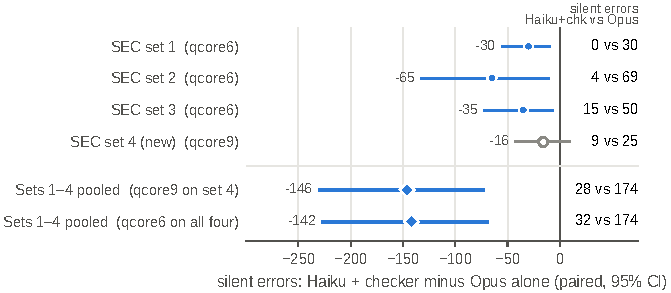
\includegraphics[width=\columnwidth]{v10_forest.pdf}
\caption{Haiku with the checker (text layer, hand identities) against Opus alone, per held-out SEC set and pooled: paired difference in silent errors with its 95\% bootstrap interval; right, the two counts. Every interval lies below zero except set~4's, where Opus alone made only 25 errors (hollow: not significant).}
\label{fig:forest}
\end{figure}


\subsection{A cheap model with the checker against the strongest model alone}\label{sec:headline}
\textbf{Set 3, frozen \vq{6}.} On set~3 Opus alone is 99.04\% accurate and leaves 50 silent errors (21--89); Haiku alone leaves 216. With \vq{6} reading the born-digital text layer, Haiku ends at 98.21\%: the checker fixed 123 of Haiku's errors from the statements' own lines, flagged 78 more (3.3\% of numbers to a person) and left 15 silent (5--28), breaking nothing. The paired difference against Opus alone is $-35$ ($-73$ to $-6$). Opus with the checker leaves 5 (0--12) of its 50, a cut of $-45$ ($-82$ to $-17$). GPT goes from 1,443 silent errors to 65 (fixing 887), not distinguishable from Opus alone ($+15$, $-32$ to $+58$), but it broke two numbers (Section~\ref{sec:allmodels}).

\textbf{Set 4, frozen \vq{9}} (Figure~\ref{fig:forest}, Table~\ref{tab:d9}). On the 24 newest filings Opus alone is 99.53\% accurate and leaves 25 silent errors (7--49), half its count on set~3; Haiku alone leaves 168 and GPT 1,090. With \vq{9} reading the text layer, Haiku leaves 9 (0--26) at 1.9\% of numbers to a person, with 124 fixes and no correct number broken. Against Opus alone that is $-16$ ($-43$ to $+10$): fewer, but not significantly; a set on which Opus errs 25 times gives the comparison little power. Strict scoring gives the same 9 against 25. Opus with the checker leaves no silent error ($-25$, $-49$ to $-7$), GPT 15 ($-1{,}075$), not distinguishable from Opus alone ($-10$, $-38$ to $+17$), with two numbers broken (Section~\ref{sec:allmodels}).

\textbf{Pooled.} Over the 227 statements of sets 1--4 (17,125 numbers), with \vq{9} on set~4 and \vq{6} on sets 1--3, Haiku plus the checker leaves 28 silent errors (10--50) against Opus alone's 174 (102--258), a paired difference of $-146$ ($-231$ to $-72$), at 2.5\% of numbers to a person and 0 broken. With \vq{6} on all four sets it leaves 32 (14--55), $-142$ ($-228$ to $-68$). Opus with the checker leaves 5; GPT 115 (126 with \vq{6} throughout) from 4,076, not distinguishable from Opus alone. Per set: 0 against 30 on set~1, 4 against 69 on set~2, 15 against 50 on set~3, all significant, and 9 against 25 on set~4.

\textbf{Hand mode is no longer version-independent.} \vq{6}, \vq{7} and \vq{8} returned the same values with hand identities on every earlier set, and \vq{8} and \vq{6} still do on set~4, in all 12 hand runs. \vq{9} returns their fixes and tier~2 items in the three no-text runs and in Opus's text run. Elsewhere its change~3 withdraws loose scaled page matches that had corroborated wrong values or held back right ones: Haiku with the text layer gets 4 more tier~2 items and its silent errors fall from 13 to 9 ($-4$, $-8$ to $-1$); each OCR run gets 1 to 5 more and loses at most one silent error; GPT with the text layer gets 3 more fixes, 14 tier~2 items more and 3 fewer, and falls from 26 to 15 ($-11$, $-23$ to 0), but breaks one more number (Appendix~\ref{app:q9}).

\textbf{Baselines} (sets 1 and 2, from an earlier version's runs on the same extractions): flagging every input of a failing identity leaves 142 silent errors; re-asking Opus on every statement with a failing identity, plus those flags, 75, breaking 25 numbers Haiku had right; using the text layer itself as the extractor, Haiku filling the rest, plus flags, 36 (20--54) at 5.0\% flagged, a baseline flattered because the truth was located on that layer. Haiku plus the checker leaves 4 there.

% Generated figure: ../gen_v10/make_figures.py (fig_allsets) from out/qcore6_heldout/results.json (sets C, ABC, D, E, F)
% and out/qcore9_heldout/results.json (set 4 = D, legacy scoring). Replaces fig_allsets6.tex. Values: ../gen_v10/figdata.json.
\begin{figure}[t]
\centering
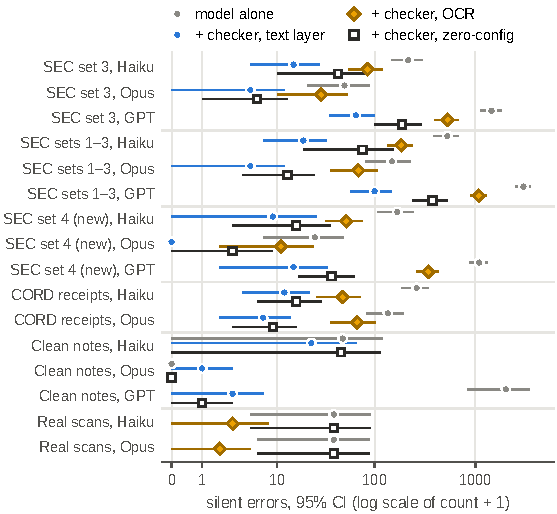
\includegraphics[width=\columnwidth]{v10_allsets.pdf}
\caption{Silent errors per held-out set and model, alone and with the checker (frozen \vq{6}; set~4: frozen \vq{9}), with 95\% bootstrap intervals; log axis of the count plus one, so 0 is the left edge. \emph{Text layer} and \emph{OCR} (docTR; real scans: the dataset's OCR) use hand identities; \emph{zero-config} uses none (real scans: no page text). With the text layer the checker cuts silent errors by one to two orders of magnitude; OCR cuts far less. Counts: Tables~\ref{tab:allsets} and~\ref{tab:d9}.}
\label{fig:allsets}
\end{figure}


\subsection{Every model gains; what broke}\label{sec:allmodels}
Over the 60 per-set (set, model, mode) settings of \vq{6} with hand identities, the checker cuts silent errors with an interval below zero in 50, and in 41 of those it broke no correct number. On set~4 \vq{9} does so in 11 of 12 hand settings, 8 with no break; the exception is Opus without page text (25 to 17). Counting discovered identities and zero-config, 26 of its 30 set-4 settings cut significantly; the four exceptions are Opus without page text. The ten exceptions are settings with almost nothing to cut: Haiku and Opus on the clean notes tables, the real scans with the scanner's OCR layer (16 and 15 silent errors fall to 1, interval touching zero), and the synthetic bundles, where the models make 0 to 2 errors. On CORD the checker cuts Haiku from 262 silent errors to 12 and Opus from 136 to 7 with the text layer, at 29.2\% and 17.0\% of numbers to a person: receipts have few identities per number, so the checker turns errors into a review queue rather than repairing them.

Twelve distinct correct numbers were broken, all silently (Table~\ref{tab:broken}). Nine came from OCR mode, where a one-glyph look-alike made an identity tie (for example a Walmart current debt, 3,542 to 4,542\,M, and an Expeditors deferred-tax line, 3.04 to 4.04\,M). Two are a pair on the new filings: in GPT's text run on a Snap-on 10-K cash flow, the period-swap repair exchanged two numbers from different rows and years (22.8 and 23.3\,M) that happened to tie the identities. One is a Salesforce debt line on the notes tables (\$39,500\,M to \$39,288\,M), broken for all three models by rule (b)'s ``extracted number printed elsewhere on its row''. No no-text run broke a number on any set, and no text run broke one on receipts, real scans or the synthetic bundles. With hand identities \vq{7} and \vq{8} return the same values, so these breaks are theirs too. On the synthetic held-out sets hand identities broke one more number, a budget figure (326 to 331) on \vq{8}'s fresh set, identically in all three versions.

Set~4 adds three numbers broken with hand identities, all silent (Appendix~\ref{app:q9}). \emph{A text layer that misprints signs}: in WAT's PDF text layer the closing parenthesis is a separate word, `(2.31' then `)', so the page shows a basic loss per share of $-2.31$ as positive; with no identity through earnings per share, rule (b) took that read in GPT's text run, in every version. This is a tokenisation gap, not a \vq{9} regression, and it causes every zero-config break on set~4 (Section~\ref{sec:zeroconfig}). \emph{A row shift, \vq{9} only}: GPT shifted a 10-K's 2024 operating cash-flow column one row; \vq{9}'s change~3 applied two correct page reads that \vq{8} had withheld, the operating sum still failed from the rest of the shift, and identity completion then finished it on the one correct cell (WST other current assets, $-5.8$ to $+5.7$\,M): net, 2 more fixes and 1 more break than \vq{8}. \emph{OCR look-alikes}: in Haiku's two OCR runs, in every version, a Domino's and a Garmin balance-sheet line were changed to the one look-alike of the OCR read that tied an identity, which had failed because another of its cells carried a Haiku error, the class of set~3's OCR breaks.

\subsection{Zero configuration}\label{sec:zeroconfig}
Table~\ref{tab:ids} (Appendix~\ref{app:q6}) runs the same data without the hand-written files. \emph{Zero-config} (no identity file, no schema) still cuts silent errors against the model alone on every SEC and CORD row: pooled SEC, Haiku 527 to 76, Opus 149 to 13, GPT 2,986 to 376 in text mode; CORD, 262 to 16 and 136 to 9. It is significant in 24 of 34 per-set settings, and its only breaks are the eight synthetic bulletin cells of Table~\ref{tab:broken}. But it is weaker than the hand identities on every SEC row: pooled Haiku leaves 76 against 19 and fixes 142 errors against 348; GPT leaves 376 against 100 and fixes 155 against 2,020; and Haiku zero-config is no longer distinguishable from Opus alone (76 against 149, $-73$, $-173$ to $+30$). The inferred schema costs more than the discovered identities: with the hand schema and discovered identities only, pooled Haiku leaves 26 and fixes 345.

Two failure modes are clear. On the real scans without page text, discovery has nothing on the page to validate against: it finds identities covering about 41\% of the numbers and they flag nothing, so the 39 silent errors stay (hand: 2 and 3). On the synthetic bulletins, discovered identities break 16 correct numbers per model (8 under zero-config), all in one age-band row, `30-34', whose label the page reader misreads and which the hand identities never let through; planted-issue routing falls from 22--24 to 8--12 of 24. Both failure modes were the targets of \vq{7} (Section~\ref{sec:q7}).

Adding the discovered identities to the hand-written ones (\emph{hand + disc.}) raises coverage on pooled SEC from 82.8\% to about 90\% and on the notes tables from 32.5\% to 61--67\%. It was never significantly worse than hand identities alone in 46 comparisons and removed the Salesforce break on the notes tables.

% Generated figure: ../gen_v10/make_figures.py (fig_setd) from out/qcore9_heldout/results.json (rows.legacy). Values: ../gen_v10/figdata.json.
\begin{figure}[t]
\centering
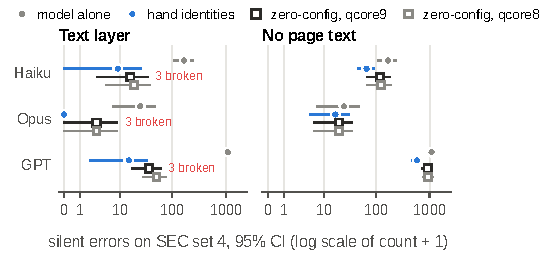
\includegraphics[width=\columnwidth]{v10_setd.pdf}
\caption{SEC set~4: the model alone, frozen \vq{9} with hand identities, and zero-config (no identity or schema file) in \vq{9} and \vq{8}; silent errors with 95\% intervals. Zero-config stays far below the model alone but above hand identities, and every zero-config text run broke the same three numbers (WAT's text layer prints the signs wrong).}
\label{fig:setd}
\end{figure}


\textbf{Set 4: the final zero-config mode on real held-out filings} (Figure~\ref{fig:setd}). The \vq{7}--\vq{9} zero-config changes had been tested held out only on synthetic data (Section~\ref{sec:q7}). On set~4, with no identity or schema file, \vq{9} leaves Haiku 16 silent errors (3--36) with the text layer, GPT 37 (17--63) and Opus 3 (0--9), against 9, 15 and 0 with hand identities and 168, 1,090 and 25 for the models alone. Haiku and GPT are significantly worse than with hand identities ($+7$, $+1$ to $+15$; $+22$, $+10$ to $+35$) but far below the model alone, and Haiku zero-config is not distinguishable from Opus alone ($-9$, $-36$ to $+17$). \vq{8} on the same inputs left 19 and 51 (GPT: $-14$, $-25$ to $-5$) and \vq{6} 31 and 113. Discovered identities covered 84.0\% of the numbers for Haiku, 88.3\% for Opus and 69.8\% for GPT, against 85.5\% for the hand files; GPT's errors leave fewer templates holding. Every zero-config text run, every model, \vq{8} and \vq{9} alike, broke the same three numbers silently: WAT's text layer shows three negative cash-flow totals ($(85)$, $(337)$, $(174)$\,M) as positive, the label read proposes sign flips, and discovered vertical sums, checked against the same misread page signs, let the flips tie. Hand identities refused them. Without page text zero-config breaks nothing but loses more: Haiku 120 against 67 with hand identities ($+53$, $+9$ to $+112$), GPT 927 against 585; \vq{9}'s new discovery cut \vq{8}'s 125 and 942 only by 5 and 15.

\subsection{\vq{7} to \vq{9} on synthetic and development data}\label{sec:q7}
% Generated figure: ../gen_v10/make_figures.py (fig_zc_versions) from out/qcore7_heldout/results.json (strict|high),
% out/qcore8_heldout/results.json (strict|all|high) and out/qcore9_heldout/results.json (legacy, Haiku). Values: ../gen_v10/figdata.json.
\begin{figure}[t]
\centering
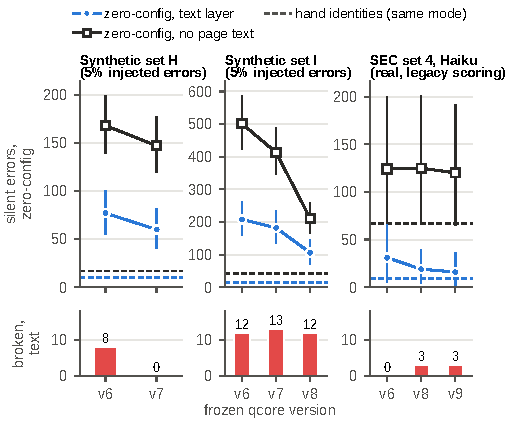
\includegraphics[width=\columnwidth]{v10_zc_versions.pdf}
\caption{Zero-config across frozen versions, each run once on a set it was not tuned on. Top: silent errors (95\% intervals) on the fresh synthetic sets H and I at the 5\% injected-error rate (strict scoring) and for Haiku on SEC set~4; dashed, hand identities in the same mode. Bottom: correct numbers broken with the text layer. Each version lowered zero-config's silent errors, most on set~I, but the gap to hand identities stays.}
\label{fig:zcversions}
\end{figure}


\textbf{Synthetic held-out sets} (Figure~\ref{fig:zcversions}; Appendices~\ref{app:q7} and~\ref{app:q8}). On \vq{7}'s fresh set \vq{7} broke no correct number where \vq{6} broke 8 with zero-config, all one age-band cell, and cut zero-config silent errors at a 5\% error rate from 77 to 60 with the text layer ($-17$, $-25$ to $-10$). On \vq{8}'s fresh set (Table~\ref{tab:q8}) zero-config \vq{8} cut \vq{7}'s silent errors by a third to a half in every setting with errors (5\% error rate: 182 to 106 with the text layer, $-76$, $-107$ to $-50$; 413 to 211 without), but left 2 to 7 times those of hand identities (106 against 15; 211 against 42). About four fifths of that gap at the high rate lay on the four new document families, which hold 71\% of the numbers, as did every zero-config break and most extra flags. It sent 7.0\% of an error-free extraction's numbers to a person with the text layer (hand 2.4\%), and broke 2, 2 and 12 correct numbers in text mode on the clean, low and high extractions: check amounts on one bank-statement layout, flipped by an inferred sign convention, and an inventory row read from its neighbour. These sets are synthetic: our generators, injected errors rather than model errors, no OCR mode, and hand identities complete by construction, which favours the hand side.

\textbf{\vq{9} on development data} (not a test). \vq{8}'s fresh set became development data, and \vq{9}'s changes 1--4 are aimed at \vq{8}'s breaks there (the bank-statement checks, the inventory row, a scaled page match behind the hand-mode budget break, a census day). The frozen development grid of the version run on set~4 (Appendix~\ref{app:q9dev}; legacy scoring, strict on sets H and I) confirms this. Zero-config \vq{9} breaks no development number, where \vq{8} broke 16 on set~I, and leaves fewer silent errors than \vq{8} on every SEC set (set~3: 1,525 to 1,460) and on sets H and I (110 to 103; 404 to 375), with at most 0.3 points more numbers to a person; the notes tables gain one silent error (95 to 96). With hand identities \vq{9} returned \vq{8}'s fixes in 350 of 352 runs and its tier~2 items in 330; the 22 that differ all read page text, and there change~3 cut silent errors on SEC set~3 from 2,304 to 2,241 and removed the set-I budget break. The regression is the CAT break above, in discovered and hand + discovered text runs (3 numbers each), which led to the refreeze. The refrozen package (freeze~2, \code{c4401b94}) fixes the CAT break on development data, with no new break (\code{out/qcore9\_work/dev\_summary9.md}); it has not been tested on held-out data.

\subsection{The re-read tier: a second read is not independent evidence}\label{sec:reread}
On development scans we asked real readers (Haiku and Opus) about crops of the unsure cells. The first gate let a re-read that agreed with an OCR digit misread change the value; it changed 11 correct SEC numbers, every one a glyph misread (16,384 to 15,384; 285,091 to 225,091) that the OCR and the reader shared. The readers repeat the extraction too: of 50 correctly placed cells where the extraction was wrong, a Haiku reader repeated the extraction's wrong number in 16 (32\%) and an Opus reader in 8 (16\%), and on 15 of Opus's 20 misreads Haiku misread the same cell. The hard glyphs on a poor scan are hard for every reader. So the frozen gate lets a re-read move a value only through an identity that then ties, and an agreeing re-read clears a flag only when the page read is another number altogether. On development scans the chosen Opus reader then cut Haiku's OCR-mode silent errors from 23 to 17 with no break.

Held out, on set~3 with docTR (Table~\ref{tab:reread}, Appendix~\ref{app:q6}), an Opus reader answered 695 crops for Haiku's extraction and 523 for Opus's. On crops placed on the right cell it was right 89\% and 85\% of the time, but where Haiku's extraction was wrong it repeated the wrong number in 13 of 70 cells. The re-reads changed no value: the fixes, and the two OCR-mode breaks, are those of the run without them. They worked only through tier~2, adding 138 and 86 \code{reread\_disagrees} items: Haiku's silent errors fell from 85 to 80 ($-5$, $-10$ to $-1$), Opus's from 29 to 27 ($-2$, $-5$ to $0$), with 0.5 and 0.2 points more numbers to a person. That moved Haiku in OCR mode from more silent errors than Opus alone ($+35$, $+3$ to $+66$) to not distinguishable ($+30$, $-3$ to $+62$), not below it. The identities, not the extra read, carry the evidence. The re-read tier was not run on set~4.

\subsection{Without a text layer the cheap model does not catch up}\label{sec:ocr}
% Generated figure: ../gen_v10/make_figures.py (fig_tradeoff) from out/qcore9_heldout/results.json (pooled_ABCD.rows: qcore6 on
% sets 1-3, qcore9 on set 4, hand identities). Values: ../gen_v10/figdata.json.
\begin{figure}[t]
\centering
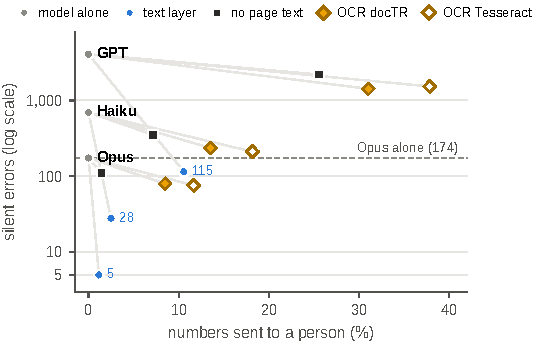
\includegraphics[width=\columnwidth]{v10_tradeoff.pdf}
\caption{Silent errors against the share of numbers sent to a person, SEC sets 1--4 pooled (17,125 numbers; hand identities, \vq{9} on set~4); thin lines join each model alone to its runs with the checker, and blue labels give the text-layer counts. Only the text layer takes the cheap model below Opus alone (dashed) at a small queue; OCR and no-text modes buy fewer silent errors with larger queues.}
\label{fig:tradeoff}
\end{figure}

% Generated figure: ../gen_v10/make_figures.py (fig_accuracy) from out/qcore9_heldout/results.json (pooled_ABCD.rows,
% accuracy and accuracy_ci). Values: ../gen_v10/figdata.json.
\begin{figure}[t]
\centering
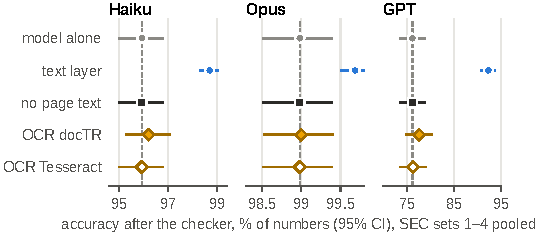
\includegraphics[width=\columnwidth]{v10_accuracy.pdf}
\caption{Accuracy after the checker by page-text mode, SEC sets 1--4 pooled, with 95\% intervals; dashed, the model alone. Fixes come from the text layer; without page text the checker writes nothing, and OCR moves it by at most one and a half points: there the gain is routing, not repair.}
\label{fig:accuracy}
\end{figure}

Figures~\ref{fig:tradeoff} and~\ref{fig:accuracy} show the pooled SEC sets by page-text mode. When the only page text is OCR of the poor scan, Haiku plus the checker leaves 184 silent errors with docTR and 172 with Tesseract on pooled sets 1--3, against Opus alone's 149 (differences $+35$, $-29$ to $+91$, and $+23$, $-45$ to $+82$); on set~3 alone the docTR run is worse than Opus alone. With no page text it leaves 285, more than Opus alone ($+136$, $+73$ to $+202$). OCR mode fixes few errors (33 of Haiku's 527); its gain is routing. The checker still helps the strong model: Opus's silent errors fall from 149 to 69 with docTR ($-80$, $-131$ to $-39$) and 62 with Tesseract, at 9.2\% and 12.4\% of numbers to a person, and from 149 to 94 with the identities alone. Set~4 repeats this with \vq{9}: Haiku plus the checker leaves 67 silent errors without page text, 52 with docTR and 39 with Tesseract, against Opus alone's 25, significantly more ($+42$, $+16$ to $+68$; $+27$, $+2$ to $+53$) or not distinguishable ($+14$, $-7$ to $+34$); Opus falls from 25 to 11 and 14 with OCR (significant) and to 17 without page text (not significant). Pooled over sets 1--4, Haiku leaves 352 without page text (Opus alone 174; $+178$, $+109$ to $+251$) and 236 and 211 with OCR, not distinguishable from Opus alone. Feeding OCR to an earlier version as if it were a text layer broke 93 (Haiku) and 102 (Opus) correct numbers on set~1 (Appendix~\ref{app:calc}); the two-reader rule removed that.

\subsection{Clean pages, real scans and synthetic documents: safety}\label{sec:safety}
\textbf{Clean notes tables.} Opus alone has no error on the 233 held-out tables; in no-text mode the checker adds neither flags nor damage, and in text mode it flags 2.1\% and breaks the Salesforce cell. Haiku's 48 errors, structural slips such as shifted columns, fall to 23 or 24, but the cut's interval touches zero: half of them lie outside every identity. GPT's 2,005 errors are 2,001 blanks; the checker names every blank and leaves 3 silent at 18.0\% of numbers to a person, a router for a model that abstains.
\textbf{Real scans.} Both models leave 39 silent errors on the 77 forms, all in the 16 forms whose annotations fail their own sums. In every run the checker changed no number; with no page text or the dataset's OCR it routed 13 (Opus) or 14 (Haiku) of the 16 and left 2 or 3 silent at 13.8--17.4\% of numbers to a person. On 33 amounts in six forms both models read the same value against the annotation, which points to annotation errors; we did not inspect the images to settle this.
\textbf{Synthetic domains.} Opus makes no error on 7,892 numbers and Haiku 2; with hand identities the checker changes no correct number, changes none of the 24 planted source-document issues, and routes 22 (Haiku) and 24 (Opus) of them.

\subsection{What made the page read safe}\label{sec:lesson}
Every time a frozen version met a new kind of document without a development step, its page reader broke correct numbers and its no-text mode broke none (Table~\ref{tab:transfer}). \vq{4} applied any own-line read that broke no tied identity, and on the notes tables, where few numbers are tied and wide tables stack period blocks over segment columns, it broke 292 of Opus's held-out numbers. The gate of Section~\ref{sec:labelread}, tuned on development tables only, cut that to the one Salesforce cell. The same lesson returned with re-reads: agreement between two readers is not enough where their errors are correlated. A change needs an identity behind it, or a cell that cannot be confused with another.

\begin{table}[t]
\centering\tsize
\caption{Correct numbers broken by tier~1 in text mode on held-out data, by the version not tuned on that kind of document and by the version tuned on its development split (per extractor for CORD, SEC and notes).}
\label{tab:transfer}
\begin{tabular*}{\columnwidth}{@{\extracolsep{\fill}}llrrr@{}}
\toprule
Held-out data & Versions & Numbers & Untuned & Tuned \\
\midrule
Synthetic domains, 24 runs & \vq{}, \vq{2} & 15,784 & 164 & 32 \\
CORD receipts & \vq{2}, \vq{3} & 998 & 157--192 & 0 \\
SEC set~1, clean & \vq{2}, \vq{3} & 2,228 & 9 & 0 \\
SEC notes tables, clean & \vq{4}, \vq{5} & 14,778 & 249--292 & 1 \\
\bottomrule
\end{tabular*}
\end{table}

\subsection{Models bend numbers so totals tie}\label{sec:bend}
The checker grew out of one for limited-partner packets from private funds (Appendix~\ref{app:pe}), where with a text layer the frozen PE checker fixed 4,685 of 4,767 model errors on held-out synthetic funds and changed no correct number. There we first saw the models bend numbers. Opus wrote: ``Where a digit was unclear, I chose the value that makes the statement's own totals add up''. On the held-out funds 398 of Opus's 423 errors tie every identity they feed (94.1\%), against 29.5\% of Haiku's, and Opus erased 10 of 13 planted source-document errors by entering consistent values (Figure~\ref{fig:example} shows Haiku making the same move on a synthetic fund). Its notes on the SEC scans read the same way: ``2026 accounts receivable: read (368) or (388). Chose (388) so operating components foot''; the page prints $(368)$. A check that only sums the extraction cannot see such a number, which is why no-text and OCR modes leave tens of Opus's errors silent, and why rule~\eqref{eq:allowed} forbids the checker the same move. Figure~\ref{fig:bend} shows both measures for the three models.

% Figure: bend-to-tie, held-out set 2, per model, with Wilson 95% intervals (paper/ci.py wilson()).
% Sources: paper/heldout2_v2.md per-run bend rows summed by model (draft.md Section 6 table):
%   own checks tie: Opus 398/423 (91.4-96.0), Haiku 454/1,539 (27.3-31.8), luna 272/2,805 (8.7-10.8)
%   erased: Opus 10/13 (49.7-91.8), Haiku 7/13 (29.1-76.8), luna 4/13 (12.7-57.6)
\begin{figure}[t]
\centering
\begin{tikzpicture}
\begin{groupplot}[group style={group size=2 by 1, horizontal sep=16pt, yticklabels at=edge left},
  dotplot, width=2.75cm, y=13pt, xmin=0, xmax=100,
  ytick={1,2,3}, ymin=1, ymax=3, y dir=reverse,
  yticklabels={Claude Opus, Claude Haiku, gpt-6-luna},
  xtick={0,50,100}, xticklabels={0,50,100\%}, enlarge y limits={abs=0.75}, title style={text height=1.6ex, text depth=0.4ex}]
\nextgroupplot[title={own checks tie}]
\addplot[dotmark, error bars/.cd, x dir=both, x explicit] coordinates {
  (94.09,1) -= (2.67,0) += (1.88,0)
  (29.50,2) -= (2.23,0) += (2.33,0)
  (9.70,3) -= (1.04,0) += (1.15,0)};
\coordinate (ben1) at (axis cs:94.09,1);
\coordinate (ben2) at (axis cs:29.50,2);
\coordinate (ben3) at (axis cs:9.70,3);
\nextgroupplot[title={planted issues erased}]
\addplot[dotmark, error bars/.cd, x dir=both, x explicit] coordinates {
  (76.92,1) -= (27.18,0) += (14.90,0)
  (53.85,2) -= (24.70,0) += (22.95,0)
  (30.77,3) -= (18.09,0) += (26.86,0)};
\coordinate (ben4) at (axis cs:76.92,1);
\coordinate (ben5) at (axis cs:53.85,2);
\coordinate (ben6) at (axis cs:30.77,3);
\end{groupplot}
\node[vlab] at (ben1) {398/423};
\node[vlab] at (ben2) {454/1,539};
\node[vlab] at (ben3) {272/2,805};
\node[vlab] at (ben4) {10/13};
\node[vlab] at (ben5) {7/13};
\node[vlab] at (ben6) {4/13};
\end{tikzpicture}
\caption{Bending to tie on the private-equity held-out set~2 (bad scans, five funds per model), with Wilson 95\% intervals. Left: share of tier~0 errors whose checks all pass on the model's own numbers. Right: share of the 13 planted document issues per model that the model's entries erased.}
\label{fig:bend}
\end{figure}



% =====================================================================
\section{Discussion}

\textbf{A recipe.} For a document set whose numbers obey linear identities, run a cheap model, then the checker; send its packets to a stronger model or a person. When the PDF keeps a born-digital text layer, this leaves fewer silent errors than the strongest model alone, at a review queue of a few percent. When the page text is OCR, run the checker behind the strongest model: it cuts silent errors by routing, but a cheap model will not catch up. On clean pages with the strongest model there is little to fix, and no-text mode costs nothing. On sparse-identity documents such as receipts, expect a review queue of 9 to 31\% of numbers.

\textbf{Cost of a new domain.} Writing the identities was the main cost of each earlier domain. Zero-config removes it at a price: on SEC statements it keeps most of the cut against the model alone but loses most of the fixes, and it needs page text to validate what it finds. \vq{7} made zero-config more cautious and \vq{8} and \vq{9} stronger; on new real filings \vq{9}'s zero-config left Haiku 16 silent errors where hand identities left 9. But on fresh synthetic layouts it still leaves several times the silent errors of hand identities and sends more numbers to a person, and each inference step (a tolerance, a label, a sign convention, a page sign) has opened a new path to a wrong change. In practice we would start zero-config, read the discovered identities (each run lists them with their support), add a hand file for the important ties, and run hand plus discovered.

\textbf{What a second opinion is worth.} The re-read result generalises beyond our checker: two vision models reading the same degraded pixels share their hard glyphs, so agreement between them is weak evidence exactly where it is needed. An identity is evidence of a different kind, because it does not look at the cell at all.

% =====================================================================
\section{Limitations}

\textbf{Text-layer dependence.} The cheap-model result needs a born-digital text layer behind the image, and that layer can be wrong: WAT's splits a closing parenthesis from its number, which caused every zero-config break on set~4. With OCR, Haiku plus the checker is not distinguishable from Opus alone on the pooled statements and is worse on sets 3 and 4 with docTR; with no page text it is worse. For CORD, text mode reads an OCR annotation that matches the truth by construction, and for SEC and the notes tables the truth was located on the same text layer that text mode reads; no-text and OCR rows are free of this.

\textbf{Identity coverage.} An error in a number no identity covers can be caught only by the page read. On the notes tables hand identities cover a third of the numbers and half of Haiku's errors lie outside them; discovered identities double the coverage there but did not reduce silent errors significantly.

\textbf{Power on set~4.} Opus alone made only 25 errors on set~4, so no comparison against it there can reach significance unless the checker's pipeline is nearly perfect; the cheap-model claim rests on set~3 and the pooled sets.

\textbf{Breaks.} With \vq{6} and hand identities twelve correct numbers were broken on sets 1--3 and the other real sets, all silently: nine by OCR look-alike repairs, which identities alone cannot tell from a coincidental tie, two by a period swap that tied by accident, and one by a page read. On set~4 \vq{9} with hand identities broke three: a misprinted page sign accepted by rule (b), a GPT row shift that change~3 helped identity completion finish on a correct cell (new in \vq{9}), and OCR look-alikes in Haiku's OCR runs; with zero-config it broke three cash-flow totals per model, every version alike, from the same misprinted signs. Zero-config \vq{6} broke eight synthetic cells on a digit-only label; \vq{8} broke 2 to 12 per extraction on its fresh synthetic set, through an inferred sign convention and an ambiguous row label; hand identities broke one synthetic budget figure in \vq{6}--\vq{8}.

\textbf{Extraction protocol.} The extraction prompt does not forbid choosing an unclear digit so that the printed totals foot, and the models' notes show they did. That lowers the errors identities can see without the page, on every SEC set alike; text mode is not affected, since it compares each cell with the page.

\textbf{The \vq{7} and \vq{8} tests} are synthetic: our own generators, injected errors, no OCR mode, and hand identities complete by construction; \vq{8} was frozen three times after development breaks before its run. The gap to hand identities is not closed (2 to 7 times on \vq{8}'s fresh set, mostly on new layouts; 16 against 9 for Haiku on set~4), and zero-config \vq{8} sends 7.0\% of an error-free extraction's numbers to a person, about three times the hand identities' share.

\textbf{Which \vq{9}.} The set-4 results are those of \vq{9}'s first freeze. The package now carries a second freeze, made after that run to fix a development break in discovery; it was not run on set~4. Its development grid found no new break; it describes its two freezes as both preceding any held-out run, which the time stamps contradict for the second.

\textbf{Re-reads.} One reader model, one OCR engine and one set were tested held out, with answers written once; crop placement follows the OCR, and 18--20\% of crops sat on another cell. Set~4 has no re-read tier.

\textbf{Scope.} Three models from two providers; GPT was not run on CORD, the real scans or the synthetic bundles. One degradation recipe for the SEC and CORD scans. The real-scan truth fails its own sums on 16 of 77 forms. Tier~2 was tested only with re-asks of Opus. SEC set~1 was seen before \vq{4} was designed. We downloaded SROIE receipts but did not evaluate on them.

% =====================================================================
\section{Conclusion}

A cheap model followed by a deterministic checker that reads the page and the documents' own identities left 15 silent errors on 22 new filings where the strongest model alone left 50, 9 against 25 on 24 further filings, run once with a version frozen before it, and 28 against 174 over 227 held-out statements; on the last set alone the gap is not significant, because the strong model erred little. Over eight held-out sets and three models the checker cut silent errors in most settings, and every number it broke is listed with its cause. It can find its identities on the page with no configuration, at a measurable cost: on the newest filings that mode left 16 silent errors for the cheap model where hand-written identities left 9, and broke three numbers per model where the filing's own text layer misprints a sign; on synthetic sets it left 2 to 7 times as many. A second model reading the same cell is correlated with the first; the identities are not, and so the rule that keeps the checker safe stays narrow: change a number only when an identity backs the page or the cell cannot be mistaken, write only what the page prints or what was extracted, and send the rest to someone who can look.

{\footnotesize
\bibliographystyle{qclosenat}
\bibliography{refs}
}

% Appendix: one-column, after the references.
\clearpage
\onecolumn
\appendix
\counterwithin{table}{section}
\newcommand{\apptab}[1]{\par\Needspace{22\baselineskip}\medskip\noindent\captionof{table}{#1}}
\small
\setlength{\tabcolsep}{5pt}

\section{Private-equity case study: details}\label{app:pe}
This appendix keeps the private-equity (PE) work the general checker grew out of, summarised in Section~\ref{sec:bend}. ``v1'' and ``v2'' are PE v1 and PE v2 of Table~\ref{tab:earlyversions}. Planted-error benches, a second real fund and planted Fund~R results from the PE-only version are not repeated here.

Each later version was checked against earlier data: \vq{} reproduces PE~v2 on the fund held-out set with no wrong change, and \vq{2}, \vq{3} and \vq{4} give identical per-error outcomes on all fund errors. On the PE validation runs \vq{5} fixes 4,687 of 4,767 errors where \vq{4} fixed 4,718 (37 fixes became tier~2 items, 6 the reverse), with no wrong change and no broken number in either.

\textbf{Data.} Fund~R is one real venture fund's packet (name withheld): 13 PDFs, 59 pages and 252 numbers, with 6 real document inconsistencies. We degraded it to image-only scans at four levels (clean 100\,dpi; scan 150\,dpi; bad\_scan 85\,dpi with tilt, noise, specks and JPEG quality 18; headless, which is bad\_scan with column headers erased), and Claude Haiku, Sonnet and Opus extracted it, 10 runs in all. The six bad\_scan and headless runs contain 193 errors. Synthetic funds come from a quarter-by-quarter fund simulator; fifteen hard funds were degraded at bad\_scan and extracted by Haiku, Opus and gpt-6-luna, in a development group and two held-out sets.

\textbf{With a text layer.} On Fund~R the frozen PE v1 fixed 189 of 193 hard-run errors (97.9\%), sent 2 to tier~2, missed 2 and made no wrong change. On held-out set~2 (funds 31--39), the frozen PE v2 fixed 4,685 of 4,767 errors (98.3\%, Wilson 95\% interval 97.9--98.6\%), sent 81 to tier~2 and missed 1. It wrote no wrong value and changed no correct number: 0 of 4,767 errors and 0 of 5,349 correct values, a one-sided 95\% upper bound of 0.06\% each. Opus alone leaves 423 of 3,372 numbers wrong there; Haiku plus tier~1 leaves 15, of which 14 are in tier~2 packets (Figure~\ref{fig:heldout2}). Without page text, v2 flags 75.3\% of these errors but only 24 of Opus's 423, because Opus's errors tie its own identities (Figure~\ref{fig:bend}). An ablation on the six Fund~R hard runs shows where the fixes come from (Figure~\ref{fig:ablation}): without the label read, tier~1 fixes 14 errors instead of 189, and arithmetic alone fixes 5, routes 124 and misses 64.

\textbf{With OCR instead of a text layer.} When we replaced the Fund~R text layer with Tesseract OCR of the degraded pages, with two safeguards (pages with median word confidence below 60 count as blank, and a number is kept only if a digits-only re-read agrees), tier~1 fixed 8 of 197 errors over nine runs and flagged 156, with no wrong change (Figure~\ref{fig:ocr}). At 85\,dpi digits are about 6\,px tall.

\textbf{Under attack.} A suite of 360 constructed cases (coordinated bending, decoy numbers, coincidental ties, planted source errors, label collisions, sign and scale traps, OCR-style digit confusions, blanks) made the frozen PE v1 write wrong values in 43 cases, all from page reads. PE v2, tuned on that suite, wrote no wrong value in either mode on 430 fresh cases generated after its freeze (upper bound 0.69\% of cases), where v1 wrote wrong values in 33 (Supplement~\ref{app:adv}). The lesson carried into the general checker: a page read must answer to the identities (the guard of Section~\ref{sec:labelread}) just as a repair does \eqref{eq:accept}.

\textbf{Bending.} On fund held-out set~2, 398 of Opus's 423 errors tie every identity they feed (94.1\%), against 454 of Haiku's 1,539 (29.5\%) and 272 of luna's 2,805. Each planted document issue fails its identities when the page is copied exactly, so if those identities tie in the extraction, the model has erased a real error in the source. Opus erased 10 of 13 planted issues (Wilson 49.7--91.8\%), Haiku 7 and luna 4.
Per-run tables of the PE work (Fund~R and synthetic-fund runs, label-read failure causes, planted errors, adversarial results per category, erased document issues), the five v1 defects with their v2 changes and four further figures are in Supplement~\ref{sup:pe}.

% Figure 2: worked repair, synthetic fund 37 (icsynth, held-out), bad_scan, Claude Haiku, Q1 2025 capital account.
% (No Opus run on a synthetic fund has a capital-account bend that a check flags: in the held-out
%  Opus runs every wrong number ties every check it feeds; see paper/heldout2_v2.md.)
% Sources (all under out/):
%   synth/fund37/bad_scan/2025 Q1/10 - Capital Account Statement.pdf   (degraded page, 85 dpi; crop rendered
%       with pdftoppm -r 255 -gray, box (195,1030)-(2007,1166) -> figures/synth_example_crop.png)
%   synth/fund37/bundle/2025 Q1/10 - Capital Account Statement.pdf     (printed text: ITD unrealized 296,477,
%       carry -50,939; ITD roll-forward 0 + 710,000 - 40,000 - 1,781 + 0 + 296,477 - 50,939 - 0 = 913,757)
%   synth/fund37/correct.jsonl   (truth: Q1 ITD unrealized 296,477, carry -50,939; Q2 unrealized QTD 618, ITD 297,095)
%   v2/synth_models/synth_fund37_haiku/text/records.jsonl  (model values: Q1 ITD unrealized 256,477, carry -10,939,
%       contributions 710,000, fees -40,000, op. income -1,781, realized 0, distributions 0, closing 913,757;
%       Q2 unrealized QTD 218, ITD 257,995)
%   v2/synth_models/synth_fund37_haiku/text/score.json     (errors, outcome "fixed", broke [])
%   model answer doc01/answer.json printed_text for carry ITD: "Allocation of carried interest -10,939 (low confidence, blurred)"
%   tier 1 = frozen v2/qclose (qclose.tiers.triage on the records above): events 256,477->296,477, -10,939->-50,939,
%       218->618, 257,995->297,095 (reason misread, "its own line on the page prints ...");
%       checks: ca.rollforward_lines.itd@2025-03-31 pass before and after (913,757);
%       xq.ca.itd_accumulates.unrealized_gain@2025-06-30 fail before (256,695 vs 257,995, diff 1,300), pass after (297,095);
%       after tier 1 no ca.* or xq.ca.* check fails.
\begin{figure}[t]
\centering
\begin{tikzpicture}[
  font=\sffamily\scriptsize,
  box/.style={draw=ink, rounded corners=1.5pt, line width=0.5pt, align=left, inner sep=3pt,
              text width=7.7cm, fill=white},
  bad/.style={box, draw=cWrong, fill=cWrong!6},
  good/.style={box, draw=cFix!80!black, fill=cFix!7},
  step/.style={font=\sffamily\scriptsize\bfseries, text=ink},
  flow/.style={-{Latex[length=1.6mm,width=1.2mm]}, line width=0.6pt, draw=ink},
  node distance=3.2pt,
]
\node[inner sep=0pt] (img) {
\includegraphics[width=8.1cm]{synth_example_crop.png}};
\node[anchor=north west, font=\sffamily\tiny, text=ink, inner sep=1pt] at ([yshift=-1pt]img.south west)
  {Q1 2025 capital account, synthetic fund 37, bad\_scan (85 dpi). Columns: ITD, YTD, QTD.};
\node[box, below=10pt of img] (b1) {%
  {\bfseries 1 Tier 0 (Haiku).} Unrealized gain ITD $=$ \textbf{256,477};\\ carried interest ITD $=$ $-$10,939.\\
  \emph{The model's note on the carry entry: ``low confidence, blurred''.}};
\node[box, below=of b1] (b2) {%
  {\bfseries 2 Q1 ITD roll-forward ties.} $710{,}000 - \dots + 256{,}477 - 10{,}939 = 913{,}757$ \textcolor{cFix!80!black}{\ding{51}}\\
  The $-40{,}000$ and $+40{,}000$ cancel, so a check inside the quarter passes.};
\node[bad, below=of b2] (b3) {%
  {\bfseries 3 Cross-quarter identity fails.} $u^{\mathrm{ITD}}_{\mathrm{Q2}} = u^{\mathrm{ITD}}_{\mathrm{Q1}} + u^{\mathrm{QTD}}_{\mathrm{Q2}}$:\\
  $256{,}477 + 218 = 256{,}695 \neq 257{,}995$, \ gap $1{,}300$ \textcolor{cWrong}{\ding{55}}};
\node[box, below=of b3] (b4) {%
  {\bfseries 4 Label read.} Each field's own line prints the value: \textbf{296,477} (ITD),\\
  carry $-$50,939; Q2 unrealized 618 (QTD) and 297,095 (ITD).};
\node[good, below=of b4] (b5) {%
  {\bfseries 5 Tier 1 writes the printed values.}\\ $256{,}477 \rightarrow 296{,}477$; \ $-10{,}939 \rightarrow -50{,}939$;\\ Q2: $218 \rightarrow 618$, $257{,}995 \rightarrow 297{,}095$\\
  $296{,}477 + 618 = 297{,}095$ \textcolor{cFix!80!black}{\ding{51}} \quad roll-forward still $913{,}757$ \textcolor{cFix!80!black}{\ding{51}}\\ every roll-forward and accumulation check on the capital accounts ties};
\end{tikzpicture}
\caption{A worked repair on a synthetic fund (held-out fund 37, bad scan, Claude Haiku; frozen v2 checker). The model entered an inception-to-date unrealized gain 40,000 below the printed value and a carried-interest charge 40,000 smaller, so the quarter's roll-forward still ties. The cross-quarter accumulation identity fails, and the fields' printed lines supply a fix that ties it; after tier 1 every roll-forward and accumulation check on the capital accounts ties.}
\label{fig:example}
\end{figure}


\apptab{PE evaluation stages, in order}\label{tab:stages}
Funds 11--19 and the 360-case suite were test data for v1 and tuning data for v2. Funds 31--39 were built (18:13 UTC) and scored with v1 (18:35) before the last v2 source edit (18:52) and the v2 freeze (19:19); the change log and the tuning outputs show that v2 was tuned only on the 360 cases and the v1 regression runs, and the fresh attack cases were generated after the freeze. This is evidence rather than enforcement.
\begin{center}
\begin{tabular}{lll}
\toprule
Stage & Data & Code; role \\
\midrule
1 Development & Fund~R runs; funds 01--09 & pre-freeze, then v1 frozen \\
2 Held-out 1 & funds 11--19, three models & v1; first test of v1 \\
3 Adversarial & 360 cases on funds 11--19 & v1; found five defects \\
4 Fixes & the 360 cases plus v1 regression runs & tuning, then v2 frozen \\
5 Held-out 2 & funds 31--39, three models & v2 (v1 also run); test of v2 \\
6 Fresh adversarial & 430 cases on funds 31--39 & v2 (v1 also run); test of v2 \\
\bottomrule
\end{tabular}
\end{center}

\section{Synthetic domains}\label{app:domains}
\apptab{Zero-shot \vq{} over all 18 synthetic-domain bundles}
Opus and Haiku read every bundle; gpt-6-luna read 16 of the 18. No-text mode broke nothing.
\begin{center}
\begin{tabular}{lrrrrrr}
\toprule
Model & Runs & Numbers & Tier 0 errors & Broken, text & Broken, no text & Tier 2 items, text \\
\midrule
Claude Opus & 18 & 11,983 & 1 & 123 & 0 & 318 \\
Claude Haiku & 18 & 11,983 & 4 & 123 & 0 & 303 \\
gpt-6-luna & 16 & 10,515 & 13 & 104 & 0 & 288 \\
\bottomrule
\end{tabular}
\end{center}

\apptab{Held-out bundles 02--05 (Opus and Haiku, 24 runs per mode): zero-shot \vq{} against frozen \vq{2}}
\begin{center}
\begin{tabular}{llrrrrrr}
\toprule
Checker & Mode & Numbers & Tier 0 errors & Broken & Tier 2 items & Planted routed & Planted changed \\
\midrule
\vq{2} & text & 15,784 & 2 & 32 & 134 & 46 / 48 & 0 \\
\vq{} & text & 15,784 & 2 & 164 & 414 & 47 / 48 & 0 \\
\vq{2} & no text & 15,784 & 2 & 0 & 83 & 46 / 48 & 0 \\
\vq{} & no text & 15,784 & 2 & 0 & 85 & 46 / 48 & 0 \\
\bottomrule
\end{tabular}
\end{center}
By domain, \vq{2} in text mode broke 0 numbers on the quarterly reports and the invoices and 32 on the bulletins, where \vq{} broke 0, 24 and 140.

\section{Held-out results of frozen \vq{6}: every set}\label{app:q6}
Frozen \vq{6} (28 files, combined sha256 {\small\nolinkurl{86debea05f95a6d2d93a7add48d32cd54e6109135052df4c1dd178c48a95ab34}}, frozen 2026-10-16T13:14:47Z; the hash matched before the runs, at their end and at report time) was run once per held-out set, model, mode and identity setting, with frozen \vq{5} re-run on the same inputs: 442 runs, none crashed, none repeated, and in every run the returned values equal the extraction plus the tier~1 fixes. The \vq{5} re-run reproduces its earlier held-out results row for row, and \vq{6} with hand identities returns exactly \vq{5}'s fixes and tier~2 items in all 104 (set, model, mode) runs, so every \vq{6}-against-\vq{5} paired difference is 0; none of \vq{6}'s default-path changes fired, because every text-mode PDF here has a born-digital text layer. On the notes tables and the real scans the checker ran over the whole bundle and rows are scored on the held-out documents. SEC set~3's extractions were checked against their locked hash manifests (132 files) before scoring, and its page images are pixel-identical to those the models read. Sources: \code{out/qcore6\_heldout/results.md}, \code{results.json}, \code{SUMMARY.md}.

\textbf{Identity settings.} \emph{Hand}: the bundle's \code{identities.json} and \code{schema.json}. \emph{Discovered}: identities discovered from the documents, hand schema. \emph{Hand + discovered}: both. \emph{Zero-config}: discovered identities and an inferred schema, neither file read. OCR modes ran with hand identities only.

\textbf{Re-read runs.} Requests were generated once for set~3, OCR mode (docTR), hand identities, for the Haiku and Opus extractions (695 and 523 requests from 914 and 634 selected cells; the rest could not be placed on a row that prints the record's label, or shared a crop). One Opus reader answered every request once (29 and 53 null answers); the answer files are hashed in \code{SUMMARY.md}. Outcomes: Haiku extraction, agrees 515, disagrees 138, another cell 56, null 32, cleared 2; Opus extraction, 377, 86, 41, 57, 2. Over all reads (crops sharing a cell counted per record), the reader gave the truth 551 of 741 times (Haiku extraction) and 386 of 561 (Opus extraction); of its errors, 12 of 158 and 3 of 118 equal the extracted value and 68 and 64 equal the OCR's page read, mostly on crops placed on another cell, where reader and OCR read the same wrong cell.

\textbf{Development data for the re-read gate} (\code{out/qcore6\_work/dev\_summary6.md}). SEC development poor scans, Haiku extraction, OCR docTR (silent / flagged / fixed / broken): no re-read 23 / 438 / 14 / 0; first gate with real Haiku answers 30 / 370 / 15 / 4; final gate, Haiku reader 19 / 449 / 14 / 0, Opus reader 17 / 449 / 14 / 0, both agreeing 19 / 445 / 14 / 0. Opus extraction: 2 / 259 / 0 / 0 without re-reads; first gate 5 / 247 / 0 / 7; final gate with the Opus reader 2 / 272 / 0 / 0. A simulated reader with independent 5\% one-digit errors had suggested 12--14 silent errors and 22--23 fixes under the first gate: real readers are worse than independent noise because their errors follow the hard glyphs.

\textbf{Natural errors on the clean notes tables} (\code{notes\_eval/scores/results.md}). Held-out: Opus 0 of 14,778; Haiku 48 (0.32\%) in 3 of 233 tables, 24 of them in numbers covered by an identity; GPT 2,005, of which 2,001 are blanks, with 99.97\% of its 12,154 non-blank answers right. Development: Opus 0 of 6,589; Haiku 16 sign errors in one table. Haiku's held-out errors are runs of values from the wrong place: a table whose columns it shifted (24 numbers), a table where every row got a different quantity (20), and four cells read from other rows.

\textbf{Set~2 silent errors of Haiku plus the checker in text mode}, the same four under \vq{3} to \vq{6}: an ABBV share repurchase read as $-1{,}496$ for $-1{,}498$\,M; a CVX share count 1,719,134 for 1,719,184; two Visa liability cells read from another row.

\textbf{Real scans: amounts where both models agree against the annotation} (\code{realscan\_eval/scores/results.md}). 33 held-out amounts in six forms: rs\_0030 (21), rs\_0008 (5), rs\_0009, rs\_0026 and rs\_0084 (2 each), rs\_0078 (1). On the 61 held-out forms whose line items sum to the gross, both models agree with every annotation.

% Generated by paper/gen_v6/gen_q6_tex.py from out/qcore6_heldout/results.json (frozen qcore6, sha256 86debea05f95a6d2...).
% v10: pointer in the caption edited by hand (moved tables are in the supplement).
\begin{table*}[t]
\centering\tsize
\caption{Every held-out set, frozen \vq{6} with the bundle's own identities, one run per set, model and mode. Each cell: silent errors (wrong at the end and named by no tier~2 item) with a 95\% bootstrap interval over documents, then the share of all numbers sent to a person (\%). $^{\dagger n}$: the run broke $n$ numbers the model had right. \emph{Text}: the checker reads the PDF's born-digital text layer while the model reads the page image (CORD: the dataset's OCR annotation). \emph{OCR}: docTR and Tesseract OCR of the same poor scan as a second reader; for the real scans, the dataset's OCR and the scanner's embedded OCR layer, the latter on the 57 forms that have one (there Haiku alone leaves 16 silent errors and Opus alone 15). --: not run. SEC sets 1 and 2 separately, and every paired difference, are in Supplement~\ref{sup:q6}.}
\label{tab:allsets}
\begin{tabular*}{\textwidth}{@{\extracolsep{\fill}}ll rr llll@{}}
\toprule
 & & \multicolumn{2}{c}{Model alone} & \multicolumn{4}{c}{Model + \vq{6}: silent [95\% CI] / \% to a person} \\
\cmidrule(lr){3-4}\cmidrule(l){5-8}
Set & Model & Acc.\,\% & Silent [95\% CI] & Text layer & No page text & OCR 1 & OCR 2 \\
\midrule
\multicolumn{8}{@{}l}{\emph{SEC set 3 (new): 22 filings, 15 10-Q and 7 10-K, poor scans of born-digital PDFs} (66 statements, 5,206 numbers)} \\
 & Haiku & 95.85 & 216 [146, 298] & 15 [5, 28] \,/\,3.3 & 123 [82, 170] \,/\,7.9 & 85 [55, 119]$^{\dagger2}$ \,/\,16.1 & 80 [53, 112]$^{\dagger1}$ \,/\,20.3 \\
 & Opus & 99.04 & 50 [21, 89] & 5 [0, 12] \,/\,1.4 & 39 [13, 75] \,/\,0.7 & 29 [10, 54] \,/\,9.9 & 25 [10, 43] \,/\,12.2 \\
 & GPT & 72.28 & 1,443 [1,120, 1,813] & 65 [35, 100]$^{\dagger2}$ \,/\,13.8 & 754 [582, 938] \,/\,29.6 & 532 [393, 684] \,/\,36.6 & 552 [423, 698]$^{\dagger1}$ \,/\,42.3 \\
\midrule
\multicolumn{8}{@{}l}{\emph{SEC sets 1--3 pooled, poor scans} (155 statements, 11,774 numbers)} \\
 & Haiku & 95.52 & 527 [388, 688] & 19 [7, 33] \,/\,2.8 & 285 [213, 365] \,/\,6.9 & 184 [135, 237]$^{\dagger2}$ \,/\,14.2 & 172 [127, 222]$^{\dagger2}$ \,/\,18.5 \\
 & Opus & 98.73 & 149 [81, 230] & 5 [0, 12] \,/\,1.2 & 94 [50, 146] \,/\,1.8 & 69 [36, 108]$^{\dagger1}$ \,/\,9.2 & 62 [31, 99] \,/\,12.4 \\
 & GPT & 74.64 & 2,986 [2,512, 3,509] & 100 [58, 148]$^{\dagger2}$ \,/\,11.0 & 1,611 [1,362, 1,871] \,/\,26.2 & 1,081 [894, 1,280]$^{\dagger2}$ \,/\,32.1 & 1,122 [940, 1,313]$^{\dagger2}$ \,/\,39.0 \\
\midrule
\multicolumn{8}{@{}l}{\emph{CORD receipts, poor scans of photos} (100 receipts, 998 numbers)} \\
 & Haiku & 73.75 & 262 [187, 344] & 12 [4, 22] \,/\,29.2 & 52 [29, 78] \,/\,25.1 & 48 [26, 73] \,/\,29.0 & 46 [24, 71] \,/\,31.1 \\
 & Opus & 86.37 & 136 [84, 194] & 7 [2, 14] \,/\,17.0 & 67 [36, 102] \,/\,8.7 & 67 [36, 102] \,/\,12.7 & 66 [36, 100] \,/\,14.8 \\
\midrule
\multicolumn{8}{@{}l}{\emph{SEC notes tables, clean pages} (233 tables, 14,778 numbers)} \\
 & Haiku & 99.68 & 48 [0, 120] & 23 [0, 66]$^{\dagger1}$ \,/\,2.3 & 24 [0, 68] \,/\,0.2 & -- & -- \\
 & Opus & 100.00 & 0 [0, 0] & 1 [0, 3]$^{\dagger1}$ \,/\,2.1 & 0 [0, 0] \,/\,0.0 & -- & -- \\
 & GPT & 86.43 & 2,005 [837, 3,403] & 3 [0, 7]$^{\dagger1}$ \,/\,19.7 & 3 [0, 7] \,/\,18.0 & -- & -- \\
\midrule
\multicolumn{8}{@{}l}{\emph{Real scanned and faxed ad-buy forms (VRDU)} (77 forms, 1,009 numbers)} \\
 & Haiku & 96.13 & 39 [5, 91] & not used & 3 [0, 8] \,/\,13.8 & 3 [0, 8] \,/\,15.1 & 1 [0, 3] \,/\,18.0 \\
 & Opus & 96.13 & 39 [6, 90] & not used & 2 [0, 5] \,/\,16.6 & 2 [0, 5] \,/\,17.4 & 1 [0, 3] \,/\,18.0 \\
\midrule
\multicolumn{8}{@{}l}{\emph{Synthetic reports, invoices and statistical bulletins} (192 documents, 7,892 numbers)} \\
 & Haiku & 99.97 & 2 [0, 5] & 2 [0, 5] \,/\,2.5 & 2 [0, 5] \,/\,1.5 & -- & -- \\
 & Opus & 100.00 & 0 [0, 0] & 0 [0, 0] \,/\,2.8 & 0 [0, 0] \,/\,1.6 & -- & -- \\
\bottomrule
\end{tabular*}
\end{table*}

% Generated by paper/gen_v6/gen_q6_tex.py from out/qcore6_heldout/results.json (frozen qcore6, sha256 86debea05f95a6d2...).
\begin{table}[t]
\centering\tsize\setlength{\tabcolsep}{2.6pt}
\caption{Where the identities come from. Silent errors, with identity coverage (share of numbers in some identity) in parentheses, for the bundle's hand-written identities, the discovered identities alone (hand schema), both, and zero-config (discovered identities and an inferred schema: no identity or schema file). $^{\dagger n}$: $n$ correct numbers broken. Every row and setting is in Appendix~\ref{app:ids}.}
\label{tab:ids}
\begin{tabular*}{\columnwidth}{@{\extracolsep{\fill}}lllrrrr@{}}
\toprule
Set & Model & Mode & Alone & Hand & Hand+disc. & Zero-config \\
\midrule
SEC 1--3 & Haiku & text & 527 & 19 (83) & 19 (91) & 76 (77) \\
SEC 1--3 & Opus & text & 149 & 5 (83) & 5 (91) & 13 (84) \\
SEC 1--3 & GPT & text & 2,986 & 100$^{\dagger2}$ (83) & 95$^{\dagger2}$ (89) & 376 (50) \\
SEC 1--3 & Haiku & no text & 527 & 285 (83) & 283 (89) & 421 (81) \\
SEC 1--3 & Opus & no text & 149 & 94 (83) & 90 (90) & 109 (87) \\
SEC 1--3 & GPT & no text & 2,986 & 1,611 (83) & 1,587 (88) & 2,482 (60) \\
\midrule
CORD & Haiku & text & 262 & 12 (72) & 12 (78) & 16 (50) \\
CORD & Opus & text & 136 & 7 (72) & 7 (79) & 9 (59) \\
\midrule
Notes & Haiku & text & 48 & 23$^{\dagger1}$ (32) & 22 (67) & 46 (56) \\
Notes & GPT & text & 2,005 & 3$^{\dagger1}$ (32) & 0 (62) & 1 (47) \\
\midrule
Real scans & Haiku & no text & 39 & 3 (99) & 3 (99) & 39 (41) \\
Real scans & Opus & no text & 39 & 2 (99) & 2 (99) & 39 (42) \\
\midrule
Synthetic & Haiku & text & 2 & 2 (98) & 2 (98) & 10$^{\dagger8}$ (81) \\
Synthetic & Opus & text & 0 & 0 (98) & 0 (98) & 8$^{\dagger8}$ (81) \\
\bottomrule
\end{tabular*}
\end{table}

% Generated by paper/gen_v6/gen_q6_tex.py from out/qcore6_heldout/results.json (rrscore, reread_vs_noreread,
% reread_requests, set C rows). Reader: one Opus reader, answers written once; extraction by Haiku or Opus; OCR docTR.
\begin{table}[t]
\centering\tsize\setlength{\tabcolsep}{3pt}
\caption{The re-read tier on SEC set~3 (OCR mode, docTR, hand identities), held out. One reader (Opus, chosen on development data) answers a crop per uncertain cell. \emph{On the cell}: the outlined cell is the record's own cell. Paired differences over documents, 95\% intervals.}
\label{tab:reread}
\begin{tabular*}{\columnwidth}{@{\extracolsep{\fill}}lrr@{}}
\toprule
 & Haiku extraction & Opus extraction \\
\midrule
Requests (per 100 numbers) & 695 (13.3) & 523 (10.0) \\
Crops on the cell / reads & 607 / 741 (82\%) & 448 / 561 (80\%) \\
Reader right, on the cell & 543 / 607 (89\%) & 379 / 448 (85\%) \\
Extraction wrong, on the cell & 70 & 12 \\
\quad reader gives the truth & 45 & 5 \\
\quad reader repeats the extraction & 13 & 3 \\
OCR wrong / reader repeats the OCR & 221 / 14 & 214 / 8 \\
\midrule
Values changed by re-reads & 0 & 0 \\
Silent, without $\rightarrow$ with & 85 $\rightarrow$ 80 & 29 $\rightarrow$ 27 \\
\quad paired difference & $-$5 [$-$10, $-$1] & $-$2 [$-$5, +0] \\
To a person, without $\rightarrow$ with & 16.1 $\rightarrow$ 16.6\% & 9.9 $\rightarrow$ 10.1\% \\
Broken, with re-reads & 2 & 0 \\
\bottomrule
\end{tabular*}
\end{table}

% Cut verbatim from appendix_q6.tex by paper/gen_v10/split_parts.py; do not edit.
\apptab{Every correct number broken by frozen \vq{6} on held-out data}\label{tab:broken}
Per-set runs only (pooled rows repeat them). Every break is silent (no tier~2 item names the cell). Reason: the tier~1 operation that made the change. The same cells broken under frozen \vq{5} on the same inputs are not repeated.
{\scriptsize\setlength{\tabcolsep}{3pt}
\begin{longtable}{l>{\raggedright\arraybackslash}p{3.3cm}>{\raggedright\arraybackslash}p{7.4cm}rrl}
\toprule
Set & Pipeline & Cell (document $|$ concept $|$ period, column) & Truth & Changed to & Reason \\
\midrule\endhead
SEC 1 & GPT + \vq{6}, OCR docTR & VZ\_2026-06-30\_cash\_flow | EmployeeBenefitsAndShareBasedCompensationNoncash | 2026-06-30 Six Months Ended June 30, 2026 & 35\,M & 30\,M & misread \\
SEC 1 & GPT + \vq{6}, OCR docTR & WMT\_2026-07-31\_balance\_sheet | LongTermDebtCurrent | 2026-01-31 January 31, 2026 & 3,542\,M & 4,542\,M & misread \\
SEC 2 & Haiku + \vq{6}, OCR Tesseract & MCD\_2026-06-30\_cash\_flow | ProceedsFromPaymentsForOtherFinancingActivities | 2025-06-30 Quarters Ended June 30, 2025 & -126\,M & -110\,M & misread \\
SEC 2 & Haiku + \vq{6} discovered ids, text & MA\_2026-06-30\_balance\_sheet | PropertyPlantAndEquipmentNet | 2026-06-30 June 30, 2026 (in millions, except per share data) & 2,541\,M & 2,756\,M & misread \\
SEC 2 & Opus + \vq{6}, OCR docTR & HON\_2026-06-30\_cash\_flow | DeferredIncomeTaxesAndTaxCredits | 2025-06-30 Six Months Ended June 30, 2025 (Dollars in millions) & -31\,M & -50\,M & misread \\
SEC 2 & GPT + \vq{6}, OCR Tesseract & DIS\_2026-06-27\_cash\_flow | IncreaseDecreaseInAccruedIncomeTaxesPayable | 2026-06-27 Nine Months Ended June 27, 2026 & -1,611\,M & -618\,M & misread \\
SEC 3 & Haiku + \vq{6}, OCR docTR & AES\_2025-12-31\_income\_statement | GeneralAndAdministrativeExpense | 2024-12-31 2024 (in millions, except per share amounts) & -288\,M & -256\,M & misread \\
SEC 3 & Haiku + \vq{6}, OCR docTR & ETSY\_2026-06-30\_cash\_flow | IncreaseDecreaseInOperatingAssetsNoncurrent | 2026-06-30 Six Months Ended June 30, 2026 & -3.239\,M & -3.25\,M & misread \\
SEC 3 & Haiku + \vq{6}, OCR Tesseract & EXPD\_2026-06-30\_balance\_sheet | DeferredIncomeTaxLiabilitiesNet | 2025-12-31 December 31, 2025 & 3.04\,M & 4.04\,M & misread \\
SEC 3 & Haiku + \vq{6}, OCR docTR + Opus re-read & AES\_2025-12-31\_income\_statement | GeneralAndAdministrativeExpense | 2024-12-31 2024 (in millions, except per share amounts) & -288\,M & -256\,M & misread \\
SEC 3 & Haiku + \vq{6}, OCR docTR + Opus re-read & ETSY\_2026-06-30\_cash\_flow | IncreaseDecreaseInOperatingAssetsNoncurrent | 2026-06-30 Six Months Ended June 30, 2026 & -3.239\,M & -3.25\,M & misread \\
SEC 3 & GPT + \vq{6}, text & SNA\_2026-01-03\_cash\_flow | AccountsReceivableAndContractReceivableCreditLossExpenseReversal | 2024-12-28 2024 & 22.8\,M & 23.3\,M & wrong\_period \\
SEC 3 & GPT + \vq{6}, text & SNA\_2026-01-03\_cash\_flow | IncreaseDecreaseInInventories | 2023-12-30 2023 & 23.3\,M & 22.8\,M & wrong\_period \\
SEC 3 & GPT + \vq{6}, OCR Tesseract & POOL\_2026-06-30\_balance\_sheet | AssetsCurrent | 2025-12-31 December 31, 2025 (Audited) & 1,969.864\,M & 1,968.964\,M & misread \\
SEC 3 & GPT + \vq{6} hand + discovered ids, text & SNA\_2026-01-03\_cash\_flow | AccountsReceivableAndContractReceivableCreditLossExpenseReversal | 2024-12-28 2024 & 22.8\,M & 23.3\,M & wrong\_period \\
SEC 3 & GPT + \vq{6} hand + discovered ids, text & SNA\_2026-01-03\_cash\_flow | IncreaseDecreaseInInventories | 2023-12-30 2023 & 23.3\,M & 22.8\,M & wrong\_period \\
Notes & Haiku + \vq{6}, text & CRM\_2026-07-31\_t036 | DebtInstrumentCarryingAmount | 2026-07-31 Outstanding Principal as of July 31, 2026 & 39,500\,M & 39,288\,M & misread \\
Notes & Opus + \vq{6}, text & CRM\_2026-07-31\_t036 | DebtInstrumentCarryingAmount | 2026-07-31 Outstanding Principal as of July 31, 2026 & 39,500\,M & 39,288\,M & misread \\
Notes & GPT + \vq{6}, text & CRM\_2026-07-31\_t036 | DebtInstrumentCarryingAmount | 2026-07-31 Outstanding Principal as of July 31, 2026 & 39,500\,M & 39,288\,M & misread \\
Synthetic & Haiku + \vq{6} discovered ids, text & public\_stats\_02 | narrative\_count | entity 30-34, 8 quarterly bulletins & 6,527--7,531 & 4,586--5,270 & misread \\
Synthetic & Haiku + \vq{6} discovered ids, text & public\_stats\_05 | narrative\_count | entity 30-34, 8 quarterly bulletins & 4,697--5,636 & 4,762--5,870 & misread \\
Synthetic & Haiku + \vq{6} zero-config, text & public\_stats\_05 | narrative\_count | entity 30-34, 8 quarterly bulletins & 4,697--5,636 & 20 & misread \\
Synthetic & Opus + \vq{6} discovered ids, text & public\_stats\_02 | narrative\_count | entity 30-34, 8 quarterly bulletins & 6,527--7,531 & 4,586--5,270 & misread \\
Synthetic & Opus + \vq{6} discovered ids, text & public\_stats\_05 | narrative\_count | entity 30-34, 8 quarterly bulletins & 4,697--5,636 & 4,762--5,870 & misread \\
Synthetic & Opus + \vq{6} zero-config, text & public\_stats\_05 | narrative\_count | entity 30-34, 8 quarterly bulletins & 4,697--5,636 & 20 & misread \\
\bottomrule
\end{longtable}}
Synthetic rows (ranges over the bulletins): the record's entity is the age band `30-34', a digit-only entity; held-out \vq{2} broke the same cells by the label read (Appendix~\ref{app:domains}). The hand identities never let the read through; discovered identities tie it.



SEC sets 1, 2 and 3, CORD, the notes tables, the real scans and the synthetic bundles separately (every run, every identity setting), and every paired difference against the model alone, against Opus alone and between identity settings, are in Supplement~\ref{sup:q6}.

\section{Frozen \vq{7} on the fresh synthetic held-out set}\label{app:q7}
Frozen \vq{7} (28 files, combined sha256 {\small\nolinkurl{51d9a35236ca553c1bd1536cee0b06c344ce06c0f0020b467613c80eb0396e55}}, frozen 2026-10-16T16:40:49Z, 65 tests) and frozen \vq{6} were run once, 2026-10-16 16:41--16:46Z, on nine bundles built with the synthetic-domain generator, imported unchanged, with new seeds (base $+$ 6, 7, 8): reports, invoices and bulletins 06--08, 144 documents, 5,920 numbers. The data were locked by a hash manifest (combined sha256 \code{6d6be8d8769f6181\dots}) at 15:27:55Z, before any \vq{7} change; the two package hashes and the data hash were checked at the start and at the end of the run. 432 runs (2 versions $\times$ 9 bundles $\times$ 3 extractions $\times$ 2 modes $\times$ 4 identity settings), none crashed. The extractions are the true values (\emph{clean}), and the true values with 89 (\emph{low}) and 297 (\emph{high}) injected errors; under strict scoring 89 and 296 numbers are wrong, under the legacy rule 81 and 278. Each extraction quotes the printed line of the PDF's text layer, as a model would. Sources: \code{out/qcore7\_heldout/SUMMARY.md}, \code{results.md}, \code{results.json}; generator of these tables: \code{paper/gen\_v7/gen\_q7\_tex.py}. Tables~\ref{tab:q7} and~\ref{tab:dev7} were in the main text of the previous version.

% Generated by paper/gen_v7/gen_q7_tex.py from out/qcore7_heldout/results.json (frozen qcore7, sha256 51d9a35236ca553c...).
\begin{table*}[t]
\centering\tsize\setlength{\tabcolsep}{2.2pt}
\caption{Frozen \vq{7} against frozen \vq{6} on the fresh synthetic held-out set (9 bundles of quarterly reports, invoices and statistical bulletins with new seeds, 144 documents, 5,920 numbers), one run. The extractions are the true values with injected errors (\emph{clean}: none; \emph{low}: 89 numbers wrong; \emph{high}: 296 wrong); no model read these pages. Strict scoring (half a printed unit). Each cell: silent errors [95\% bootstrap interval over documents] / \% of numbers to a person (discovered identities with the hand schema: silent only); $^{\dagger n}$: $n$ correct numbers broken. \emph{Hand, both}: hand identities, where the two versions return the same fixes and tier~2 items in all 54 runs. Paired differences over the same resamples. Every row, the legacy scoring and every broken number: Appendix~\ref{app:q7}.}
\label{tab:q7}
\begin{tabular*}{\textwidth}{@{\extracolsep{\fill}}ll r l ll ll ll@{}}
\toprule
 & & & & \multicolumn{2}{c}{Discovered ids (silent)} & \multicolumn{2}{c}{Zero-config} & \multicolumn{2}{c}{Zero-config, paired silent diff.} \\
\cmidrule(lr){5-6}\cmidrule(lr){7-8}\cmidrule(l){9-10}
Extraction & Mode & Alone & Hand, both & \vq{6} & \vq{7} & \vq{6} & \vq{7} & \vq{7} $-$ \vq{6} & \vq{7} $-$ hand \\
\midrule
clean & text & 0 & 0 [0, 0] / 2.9 & 16$^{\dagger16}$ & 0 & 8 [3, 14]$^{\dagger8}$ / 2.0 & 0 [0, 0] / 2.4 & $-$8 [$-$14, $-$3] & 0 [0, 0] \\
 & no text &  & 0 [0, 0] / 1.4 & 0 & 0 & 0 [0, 0] / 0.6 & 0 [0, 0] / 0.6 & 0 [0, 0] & 0 [0, 0] \\
\addlinespace[2pt]
low, 1.5\% & text & 89 & 5 [1, 10] / 5.5 & 32$^{\dagger16}$ & 14 & 26 [17, 35]$^{\dagger8}$ / 4.2 & 15 [8, 23] / 4.9 & $-$11 [$-$18, $-$5] & +10 [+4, +16] \\
 & no text &  & 6 [2, 11] / 7.2 & 32 & 27 & 32 [21, 44] / 4.0 & 27 [17, 38] / 4.9 & $-$5 [$-$11, 0] & +21 [+13, +30] \\
\addlinespace[2pt]
high, 5\% & text & 296 & 10 [4, 18] / 13.4 & 77$^{\dagger15}$ & 54 & 77 [56, 100]$^{\dagger8}$ / 7.7 & 60 [41, 81] / 8.5 & $-$17 [$-$25, $-$10] & +50 [+32, +69] \\
 & no text &  & 17 [8, 27] / 20.5 & 168 & 147 & 168 [140, 198] / 7.7 & 147 [120, 176] / 8.8 & $-$21 [$-$32, $-$11] & +130 [+104, +157] \\
\bottomrule
\end{tabular*}
\end{table*}

% Cut verbatim from appendix_q7.tex by paper/gen_v10/split_parts.py; do not edit.
\apptab{Every correct number broken on the fresh held-out set (strict)}\label{tab:q7broken}
\vq{7} broke none in any of its 24 settings. Every \vq{6} break is silent and is the age band `30-34' of the births bulletins (field \code{narrative\_count}, one cell per quarterly bulletin), read by the label read as a value.
\begin{center}\footnotesize
\begin{tabular}{lllrl}
\toprule
Extraction & Pipeline & Bundles (cells) & Broken & Changed to \\
\midrule
clean & \vq{6} discovered, text & public\_stats\_06 (8), public\_stats\_07 (8) & 16 & 5,585--7,814 \\
clean & \vq{6} zero-config, text & public\_stats\_07 (8) & 8 & 20 \\
low, 1.5\% & \vq{6} discovered, text & public\_stats\_06 (8), public\_stats\_07 (8) & 16 & 5,585--7,814 \\
low, 1.5\% & \vq{6} zero-config, text & public\_stats\_07 (8) & 8 & 20 \\
high, 5\% & \vq{6} discovered, text & public\_stats\_06 (7), public\_stats\_07 (8) & 15 & 5,725--7,814 \\
high, 5\% & \vq{6} zero-config, text & public\_stats\_07 (8) & 8 & 20 \\
\bottomrule
\end{tabular}
\end{center}



Every run, the paired differences, legacy scoring, injected errors by kind and by domain, and \vq{7}'s development grid are in Supplement~\ref{sup:q7}.

\section{Frozen \vq{9} on SEC set~4 (set D)}\label{app:q9}
Frozen \vq{9} (30 files, combined sha256 {\small\nolinkurl{3ca510d3ea178550ee3a43676d9f8e74a4e4ec0c4e4e8b7d4149d72732d387e0}}, frozen 2026-10-18T18:27:04Z, 79 tests; the package's first freeze, see below), frozen \vq{8} and frozen \vq{6} were run once, 2026-10-18 18:40--19:19Z, on SEC set~4 (\code{sec\_eval4}): 24 filings (16 10-Qs, 8 10-Ks; ALB, CF, CLX, CTAS, DPZ, EXR, FAST, GRMN, HSY, JBHT, KMB, LKQ, LULU, MLM, NDSN, PAYX, ROL, STE, TER, TSCO, ULTA, WAT, WST, ZBRA), 72 statements, 5,351 located facts (USD 5,023, per share 207, shares 121), 1,135 identities (998 from calculation linkbases, for six filers read from the linkbase embedded in the schema file; all hold on the truth; 9 failing linkbase relations excluded before writing). The bundles and page images were locked at 15:43:59Z (manifests \code{0b37a250\dots}, 76 files; \code{ba82b969\dots}, 152 files), the Haiku and Opus extractions at 15:54Z (\code{6ae22d31\dots}, 263 files) and GPT's at 16:12Z (\code{7156d227\dots}, 72 files), all before the freeze; the four manifests and the three package hashes were verified before the runs, after them and at report time. 90 runs (3 versions $\times$ 3 models $\times$ hand identities in four modes and three discovered settings in two), none crashed, none repeated, in three batches because OCR was not ready (text and no text 72 runs, Tesseract 9, docTR 9). OCR used \vq{9}'s \code{ocr} command, whose file is identical to \vq{6}'s, on page images pixel-identical to those the models read. The extractions were made as for set~3, by subagents, 12 batches of six statements per model, with set~3's prompt; Haiku left 2 blanks, Opus 0, GPT 10. The prompt does not forbid using printed totals to settle an unclear digit; of the per-statement notes (Haiku 67, Opus 52), 40 and 38 mention footing. The Opus re-read tier, run on set~3 as an add-on row, was not run. Scoring: legacy (primary, as sets 1--3) and strict (half a printed unit). Runtimes in the run records are inflated: \vq{9}'s development grid shared the machine. Sources: \code{out/qcore9\_heldout/SUMMARY.md}, \code{results.md}, \code{results.json}, \code{notes.json}; \code{sec\_eval4/README.md}; \code{qcore9/CHANGES.md}; generator of these tables: \code{paper/gen\_v9/gen\_q9\_tex.py}. \emph{Refreeze.} At 19:59:26Z, after this run, \vq{9} was refrozen (\code{c4401b943fcb8eb1\dots}; \code{qcore9/frozen\_manifest.json} and \code{out/qcore9\_work/FROZEN.md} now name that hash) because the first freeze's development grid broke one SEC development number in discovered-identity runs; \code{auto.\_one\_slip} now needs a digit change of two units or more. The record says both freezes preceded any held-out run; the run records above (package checks 18:40:54Z, 19:19:23Z and 19:23:34Z, all \code{3ca510d3}) show the second came after this run. The change is in discovery only, so the hand-identity rows would be unchanged; the discovered and zero-config rows are those of the first freeze.

% Generated by paper/gen_v9/gen_q9_tex.py from out/qcore9_heldout/results.json (frozen qcore9, sha256 3ca510d3ea178550...).
% v10: pointer in the caption edited by hand (moved tables are in the supplement).
\begin{table*}[t]
\centering\tsize\setlength{\tabcolsep}{1.5pt}
\caption{\textbf{SEC set~4} (set D in the result files): 24 new filings, 16 10-Qs and 8 10-Ks, 72 statements, 5,351 numbers, poor scans of born-digital PDFs; frozen \vq{9}, one run. Cells: silent errors (with the text layer, and for the model alone, with a 95\% bootstrap interval over statements) / \% of numbers to a person; $^{\dagger n}$: $n$ numbers the model had right were broken. Hand: the bundle's identities and schema; ZC: zero-config, no identity or schema file (\vq{8} on the same inputs in parentheses). Lower block: sets 1--4 pooled with hand identities; sets 1--3 are \vq{6}'s frozen held-out runs re-scored (they reproduce its results in all 137 rows), set~4 is \vq{6} (\emph{all \vq{6}}) or \vq{9}; Opus rows are the same both ways. Legacy scoring. Paired differences: Table~\ref{tab:q9paired}; every run, with the \vq{8} and \vq{6} re-runs: Supplement~\ref{sup:q9}.}
\label{tab:d9}
\begin{tabular*}{\textwidth}{@{\extracolsep{\fill}}l rr llll ll@{}}
\toprule
 & \multicolumn{2}{c}{Model alone} & \multicolumn{4}{c}{Model + \vq{9}, hand identities} & \multicolumn{2}{c}{Model + \vq{9}, zero-config (\vq{8})} \\
\cmidrule(lr){2-3}\cmidrule(lr){4-7}\cmidrule(l){8-9}
Model & Acc.\,\% & Silent [CI] & Text layer & No page text & docTR & Tesseract & Text layer & No page text \\
\midrule
\multicolumn{9}{@{}l}{\emph{SEC set 4 (new, held out): 72 statements, 5,351 numbers}} \\
Haiku & 96.86 & 168 [108, 246] & 9 [0, 26] / 1.9 & 67 / 7.8 & 52$^{\dagger1}$ / 12.0 & 39$^{\dagger1}$ / 17.4 & 16 [3, 36]$^{\dagger3}$ / 2.5 (19) & 120 / 4.3 (125) \\
Opus & 99.53 & 25 [7, 49] & 0 [0, 0] / 1.0 & 17 / 0.7 & 11 / 7.0 & 14 / 10.1 & 3 [0, 9]$^{\dagger3}$ / 1.2 (3) & 20 / 1.1 (20) \\
GPT & 79.63 & 1,090 [874, 1,324] & 15 [2, 34]$^{\dagger2}$ / 9.6 & 585 / 24.1 & 343 / 28.6 & 408 / 35.3 & 37 [17, 63]$^{\dagger3}$ / 14.9 (51) & 927 / 9.7 (942) \\
\midrule
\multicolumn{9}{@{}l}{\emph{SEC sets 1--4 pooled, hand identities: 227 statements, 17,125 numbers}} \\
Haiku, all \vq{6} & 95.94 & 695 [536, 867] & 32 [14, 55] / 2.5 & 352 / 7.2 & 237$^{\dagger3}$ / 13.5 & 211$^{\dagger3}$ / 18.2 & -- & -- \\
\quad \vq{9} on set 4 &  &  & 28 [10, 50] / 2.5 & 352 / 7.2 & 236$^{\dagger3}$ / 13.5 & 211$^{\dagger3}$ / 18.2 & -- & -- \\
Opus & 98.98 & 174 [102, 258] & 5 [0, 12] / 1.2 & 111 / 1.4 & 80$^{\dagger1}$ / 8.5 & 76 / 11.7 & -- & -- \\
GPT, all \vq{6} & 76.20 & 4,076 [3,536, 4,629] & 126 [82, 176]$^{\dagger3}$ / 10.6 & 2,196 / 25.5 & 1,425$^{\dagger2}$ / 31.0 & 1,530$^{\dagger2}$ / 37.8 & -- & -- \\
\quad \vq{9} on set 4 &  &  & 115 [71, 166]$^{\dagger4}$ / 10.6 & 2,196 / 25.5 & 1,424$^{\dagger2}$ / 31.0 & 1,530$^{\dagger2}$ / 37.8 & -- & -- \\
\bottomrule
\end{tabular*}
\end{table*}

% Cut verbatim from appendix_q9.tex by paper/gen_v10/split_parts.py; do not edit.
\apptab{Paired differences in silent errors, \vq{9} on SEC set~4 (legacy), sums over statements, 95\% bootstrap intervals}\label{tab:q9paired}
\emph{vs alone}: against the same model alone; \emph{vs Opus alone} (Haiku and GPT): against Opus alone (25 silent errors); \emph{vs \vq{8}, vs \vq{6}}: the same model, mode and identity setting; \emph{vs hand}: discovered against hand identities, \vq{9}. 10,000 resamples, seed 0.
{\scriptsize\setlength{\tabcolsep}{3pt}
\begin{longtable}{lllrlllll}
\toprule
Model & Mode & Identities & Silent & vs alone & vs Opus alone & vs \vq{8} & vs \vq{6} & vs hand \\
\midrule\endhead
Haiku & text & hand & 9 & $-$159 [$-$237, $-$100] & $-$16 [$-$43, +10] & $-$4 [$-$8, $-$1] & $-$4 [$-$8, $-$1] & -- \\
Haiku & text & discovered & 13 & $-$155 [$-$234, $-$95] & $-$12 [$-$40, +15] & $-$3 [$-$7, 0] & $-$3 [$-$9, +3] & +4 [0, +11] \\
Haiku & text & hand + disc. & 9 & $-$159 [$-$237, $-$100] & $-$16 [$-$43, +10] & $-$4 [$-$8, $-$1] & $-$4 [$-$8, $-$1] & 0 [0, 0] \\
Haiku & text & zero-config & 16 & $-$152 [$-$229, $-$94] & $-$9 [$-$36, +17] & $-$3 [$-$7, 0] & $-$15 [$-$44, +3] & +7 [+1, +15] \\
Haiku & no text & hand & 67 & $-$101 [$-$166, $-$52] & +42 [+16, +68] & 0 [0, 0] & 0 [0, 0] & -- \\
Haiku & no text & discovered & 120 & $-$48 [$-$65, $-$33] & +95 [+52, +148] & $-$4 [$-$9, 0] & $-$5 [$-$11, $-$1] & +53 [+9, +112] \\
Haiku & no text & hand + disc. & 56 & $-$112 [$-$177, $-$63] & +31 [+6, +56] & 0 [0, 0] & 0 [0, 0] & $-$11 [$-$21, $-$3] \\
Haiku & no text & zero-config & 120 & $-$48 [$-$65, $-$33] & +95 [+52, +148] & $-$5 [$-$11, $-$1] & $-$4 [$-$9, 0] & +53 [+9, +112] \\
Haiku & OCR docTR & hand & 52 & $-$116 [$-$183, $-$66] & +27 [+2, +53] & $-$1 [$-$3, 0] & $-$1 [$-$3, 0] & -- \\
Haiku & OCR Tesseract & hand & 39 & $-$129 [$-$196, $-$77] & +14 [$-$7, +34] & 0 [0, 0] & 0 [0, 0] & -- \\
\midrule
Opus & text & hand & 0 & $-$25 [$-$49, $-$7] & -- & 0 [0, 0] & 0 [0, 0] & -- \\
Opus & text & discovered & 3 & $-$22 [$-$46, $-$3] & -- & 0 [0, 0] & +1 [$-$3, +6] & +3 [0, +9] \\
Opus & text & hand + disc. & 0 & $-$25 [$-$49, $-$7] & -- & 0 [0, 0] & 0 [0, 0] & 0 [0, 0] \\
Opus & text & zero-config & 3 & $-$22 [$-$46, $-$3] & -- & 0 [0, 0] & +2 [$-$3, +9] & +3 [0, +9] \\
Opus & no text & hand & 17 & $-$8 [$-$22, 0] & -- & 0 [0, 0] & 0 [0, 0] & -- \\
Opus & no text & discovered & 20 & $-$5 [$-$12, 0] & -- & 0 [0, 0] & 0 [0, 0] & +3 [0, +9] \\
Opus & no text & hand + disc. & 17 & $-$8 [$-$22, 0] & -- & 0 [0, 0] & 0 [0, 0] & 0 [0, 0] \\
Opus & no text & zero-config & 20 & $-$5 [$-$12, 0] & -- & 0 [0, 0] & 0 [0, 0] & +3 [0, +9] \\
Opus & OCR docTR & hand & 11 & $-$14 [$-$29, $-$3] & -- & 0 [0, 0] & 0 [0, 0] & -- \\
Opus & OCR Tesseract & hand & 14 & $-$11 [$-$26, $-$2] & -- & 0 [0, 0] & 0 [0, 0] & -- \\
\midrule
GPT & text & hand & 15 & $-$1,075 [$-$1,303, $-$863] & $-$10 [$-$38, +17] & $-$11 [$-$23, 0] & $-$11 [$-$23, 0] & -- \\
GPT & text & discovered & 27 & $-$1,063 [$-$1,291, $-$853] & +2 [$-$28, +30] & $-$11 [$-$20, $-$4] & $-$15 [$-$25, $-$7] & +12 [+3, +23] \\
GPT & text & hand + disc. & 15 & $-$1,075 [$-$1,302, $-$864] & $-$10 [$-$38, +17] & $-$9 [$-$20, +1] & $-$10 [$-$21, 0] & 0 [$-$4, +4] \\
GPT & text & zero-config & 37 & $-$1,053 [$-$1,278, $-$845] & +12 [$-$18, +43] & $-$14 [$-$25, $-$5] & $-$76 [$-$138, $-$33] & +22 [+10, +35] \\
GPT & no text & hand & 585 & $-$505 [$-$667, $-$362] & +560 [+443, +693] & 0 [0, 0] & 0 [0, 0] & -- \\
GPT & no text & discovered & 927 & $-$163 [$-$202, $-$127] & +902 [+705, +1,117] & $-$19 [$-$37, $-$6] & $-$32 [$-$53, $-$15] & +342 [+206, +497] \\
GPT & no text & hand + disc. & 554 & $-$536 [$-$698, $-$391] & +529 [+415, +657] & $-$7 [$-$17, $-$1] & $-$8 [$-$21, +5] & $-$31 [$-$48, $-$13] \\
GPT & no text & zero-config & 927 & $-$163 [$-$202, $-$127] & +902 [+705, +1,117] & $-$15 [$-$25, $-$6] & $-$28 [$-$45, $-$14] & +342 [+206, +497] \\
GPT & OCR docTR & hand & 343 & $-$747 [$-$929, $-$582] & +318 [+241, +406] & $-$1 [$-$3, 0] & $-$1 [$-$3, 0] & -- \\
GPT & OCR Tesseract & hand & 408 & $-$682 [$-$854, $-$526] & +383 [+290, +489] & 0 [0, 0] & 0 [0, 0] & -- \\
\bottomrule
\end{longtable}}


% Cut verbatim from appendix_q9.tex by paper/gen_v10/split_parts.py; do not edit.
\apptab{SEC sets 1--4 pooled, hand identities (legacy)}\label{tab:q9pooled}
17,125 numbers, 227 statements (sets 1--3: 11,774 numbers, frozen \vq{6} held-out runs re-scored; they reproduce \code{out/qcore6\_heldout/results.json} in 137 of 137 rows). \emph{all \vq{6}}: \vq{6} on set~4 too (comparable with the pooled rows of earlier versions); \emph{\vq{9} on set 4}: \vq{6} on sets 1--3 and \vq{9} on set~4. Differences against Opus alone are paired over statements.
\begin{center}\footnotesize
\begin{tabular}{lllrrl}
\toprule
Model & Mode & Set 4 & Silent [CI] & To a person & vs Opus alone \\
\midrule
Haiku & alone & & 695 [536, 867] & 0.0\% & \\
Haiku & text & all \vq{6} & 32 [14, 55] & 2.5\% & $-$142 [$-$228, $-$68] \\
Haiku & text & \vq{9} & 28 [10, 50] & 2.5\% & $-$146 [$-$231, $-$72] \\
Haiku & no text & all \vq{6} & 352 [276, 438] & 7.2\% & +178 [+109, +251] \\
Haiku & no text & \vq{9} & 352 [276, 438] & 7.2\% & +178 [+109, +251] \\
Haiku & OCR docTR & all \vq{6} & 237 [183, 295]$^{\dagger3}$ & 13.5\% & +63 [$-$5, +125] \\
Haiku & OCR docTR & \vq{9} & 236 [182, 294]$^{\dagger3}$ & 13.5\% & +62 [$-$5, +124] \\
Haiku & OCR Tesseract & all \vq{6} & 211 [161, 266]$^{\dagger3}$ & 18.2\% & +37 [$-$32, +100] \\
Haiku & OCR Tesseract & \vq{9} & 211 [161, 266]$^{\dagger3}$ & 18.2\% & +37 [$-$32, +100] \\
\midrule
Opus & alone & & 174 [102, 258] & 0.0\% & \\
Opus & text & all \vq{6} & 5 [0, 12] & 1.2\% &  \\
Opus & text & \vq{9} & 5 [0, 12] & 1.2\% &  \\
Opus & no text & all \vq{6} & 111 [64, 166] & 1.4\% &  \\
Opus & no text & \vq{9} & 111 [64, 166] & 1.4\% &  \\
Opus & OCR docTR & all \vq{6} & 80 [44, 123]$^{\dagger1}$ & 8.5\% &  \\
Opus & OCR docTR & \vq{9} & 80 [44, 123]$^{\dagger1}$ & 8.5\% &  \\
Opus & OCR Tesseract & all \vq{6} & 76 [43, 117] & 11.7\% &  \\
Opus & OCR Tesseract & \vq{9} & 76 [43, 117] & 11.7\% &  \\
\midrule
GPT & alone & & 4,076 [3,536, 4,629] & 0.0\% & \\
GPT & text & all \vq{6} & 126 [82, 176]$^{\dagger3}$ & 10.6\% & $-$48 [$-$143, +38] \\
GPT & text & \vq{9} & 115 [71, 166]$^{\dagger4}$ & 10.6\% & $-$59 [$-$153, +28] \\
GPT & no text & all \vq{6} & 2,196 [1,921, 2,490] & 25.5\% & +2,022 [+1,769, +2,290] \\
GPT & no text & \vq{9} & 2,196 [1,921, 2,490] & 25.5\% & +2,022 [+1,769, +2,290] \\
GPT & OCR docTR & all \vq{6} & 1,425 [1,224, 1,639]$^{\dagger2}$ & 31.0\% & +1,251 [+1,069, +1,449] \\
GPT & OCR docTR & \vq{9} & 1,424 [1,223, 1,638]$^{\dagger2}$ & 31.0\% & +1,250 [+1,068, +1,448] \\
GPT & OCR Tesseract & all \vq{6} & 1,530 [1,331, 1,745]$^{\dagger2}$ & 37.8\% & +1,356 [+1,166, +1,559] \\
GPT & OCR Tesseract & \vq{9} & 1,530 [1,331, 1,745]$^{\dagger2}$ & 37.8\% & +1,356 [+1,166, +1,559] \\
\bottomrule
\end{tabular}
\end{center}


% Cut verbatim from appendix_q9.tex by paper/gen_v10/split_parts.py; do not edit.
\apptab{Every correct number broken on SEC set~4 (legacy; strict breaks the same numbers), with its cause}\label{tab:q9broken}
Each cell once, with every run that broke it ($^{f}$: flagged in that run; all others silent). No no-text run broke a number. Causes: (1) WAT's PDF text layer prints the closing parenthesis as a separate word, so a negative number reads as positive (a tokenisation gap in every version); (2) a GPT row shift that \vq{9}'s change~3 partly repaired and identity completion then finished on a correct cell; (3) OCR look-alike repairs, the class of set~3's OCR breaks; (4) a \vq{6} discovery break fixed in \vq{7}.
{\scriptsize\setlength{\tabcolsep}{3pt}
\begin{longtable}{p{4.6cm}rrlp{8.2cm}}
\toprule
Cell & Truth & Changed to & Cause & Runs that broke it \\
\midrule\endhead
WAT cash flow: Net cash used in financing activities (2025) & -174,000,000 & 174,000,000 & (1) & Haiku q9 disc., text; Haiku q9 ZC, text; Haiku q8 disc., text; Haiku q8 ZC, text; Haiku q6 disc., text$^{f}$; Opus q9 disc., text; Opus q9 ZC, text; Opus q8 disc., text; Opus q8 ZC, text; Opus q6 disc., text$^{f}$; GPT q9 disc., text; GPT q9 ZC, text; GPT q8 disc., text; GPT q8 ZC, text; GPT q6 disc., text \\
WAT cash flow: Net cash used in financing activities (2026) & -337,000,000 & 337,000,000 & (1) & Haiku q9 disc., text; Haiku q9 ZC, text; Haiku q8 disc., text; Haiku q8 ZC, text; Haiku q6 disc., text; Opus q9 disc., text; Opus q9 ZC, text; Opus q8 disc., text; Opus q8 ZC, text; Opus q6 disc., text; GPT q9 disc., text; GPT q9 ZC, text; GPT q8 disc., text; GPT q8 ZC, text; GPT q6 disc., text \\
WAT cash flow: Net cash provided by (used in) investing activities (2025) & -85,000,000 & 85,000,000 & (1) & Haiku q9 disc., text; Haiku q9 ZC, text; Haiku q8 disc., text; Haiku q8 ZC, text; Haiku q6 disc., text$^{f}$; Opus q9 disc., text; Opus q9 ZC, text; Opus q8 disc., text; Opus q8 ZC, text; Opus q6 disc., text$^{f}$; GPT q9 disc., text; GPT q9 ZC, text; GPT q8 disc., text; GPT q8 ZC, text; GPT q6 disc., text \\
WAT income statement: Net (loss) income per basic common share (2026) & -2.31 & 2.31 & (1) & GPT q9, text; GPT q8, text; GPT q6, text; GPT q6 disc., text; GPT q6 hand+disc., text \\
WST cash flow: Decrease (increase) in other current assets (2024) & -5,800,000 & 5,700,000 & (2) & GPT q9, text; GPT q9 hand+disc., text \\
DPZ balance sheet: Advertising fund assets, restricted (2024) & 103,396,000 & 103,316,000 & (3) & Haiku q9, docTR; Haiku q8, docTR; Haiku q6, docTR \\
GRMN balance sheet: Deferred income tax assets (2024) & 822,521,000 & 822,623,000 & (3) & Haiku q9, Tess.; Haiku q8, Tess.; Haiku q6, Tess. \\
ALB balance sheet: Common stock, \$.01 par value, \dots (2025) & 1,178,000 & 2,025,000 & (4) & Haiku q6 disc., text; Opus q6 disc., text; GPT q6 disc., text \\
\bottomrule
\end{longtable}}



Every run of \vq{9}, \vq{8} and \vq{6} on set~4 and the run-by-run hand-identity check are in Supplement~\ref{sup:q9}.

\section{Development grid of frozen \vq{9}}\label{app:q9dev}
% Cut verbatim from appendix_q9dev.tex by paper/gen_v10/split_parts.py; do not edit.
% Generated by paper/gen_v9/gen_dev9.py from out/qcore9_work/dev_report9.json (DEV grid, frozen qcore9 3ca510d3ea178550...).
\textbf{The grid of the version run on set~4.} This is the development grid of \vq{9}'s first freeze (\code{3ca510d3}), the version run on set~4, copied before the package was refrozen (\code{/home/claude/q9/logs/dev\_report9\_freeze1.json}, \code{.md}; written by \code{out/qcore9\_work/dev\_report9.py}). Its one new break, CAT's six-month net income to common holders (6,142 to 6,141\,M) in discovered and hand + discovered text runs of the SEC development filings, led to the refreeze (Section~\ref{sec:protocol}). Set names are those of the development scripts: A, B, C = SEC sets 1--3; D = CORD test; E = notes tables; F = real scans; G = synthetic 02--05; H, I = \vq{7}'s and \vq{8}'s fresh sets. \textbf{Development data only.} Every set below was spent before \vq{9} was written, and \vq{9} was tuned on them, set~I (\vq{8}'s fresh set) included. Frozen \vq{9} was run on every (set, model, extraction, mode, identity setting) of the grid; the \vq{8} runs are \vq{8}'s own frozen grid and, for set~I, its held-out run. Hand-identity check, run by run: 352 hand runs, 350 with \vq{8}'s fixes, 330 with its tier~2 items (22 differ, all through change~3). Missing runs: 0. 
% Generated by paper/gen_v9/gen_dev9.py from out/qcore9_work/dev_report9.json (DEV grid, frozen qcore9 3ca510d3ea178550... vs frozen qcore8).
\begin{table}[h]
\centering\footnotesize\setlength{\tabcolsep}{4pt}
\caption{\textbf{Development data}, not held out: frozen \vq{8} $\rightarrow$ \vq{9}'s first freeze (the version run on set~4) on every spent set, pooled over models, extractions and modes; legacy scoring, strict for sets H and I. \vq{9} was tuned on these sets. Hand identities: 350 of 352 runs return \vq{8}'s fixes and 330 its tier~2 items. Every row: Appendix~\ref{app:q9dev}.}
\label{tab:dev9}
\begin{tabular}{llrrrr}
\toprule
Set & Ids & Silent & Broken & Fixed & Flag.\,\% \\
\midrule
SEC set 1 & hand & 885 $\rightarrow$ 885 & 2 $\rightarrow$ 2 & 563 $\rightarrow$ 563 & 14.3 $\rightarrow$ 14.4 \\
SEC set 1 & ZC & 593 $\rightarrow$ 575 & 0 $\rightarrow$ 0 & 259 $\rightarrow$ 284 & 6.0 $\rightarrow$ 6.3 \\
SEC set 2 & hand & 1,615 $\rightarrow$ 1,614 & 3 $\rightarrow$ 3 & 1,001 $\rightarrow$ 1,001 & 12.9 $\rightarrow$ 12.9 \\
SEC set 2 & ZC & 1,072 $\rightarrow$ 1,054 & 0 $\rightarrow$ 0 & 381 $\rightarrow$ 406 & 6.1 $\rightarrow$ 6.3 \\
SEC set 3 & hand & 2,304 $\rightarrow$ 2,241 & 6 $\rightarrow$ 6 & 1,108 $\rightarrow$ 1,108 & 16.2 $\rightarrow$ 16.3 \\
SEC set 3 & ZC & 1,525 $\rightarrow$ 1,460 & 0 $\rightarrow$ 0 & 449 $\rightarrow$ 473 & 8.0 $\rightarrow$ 8.3 \\
CORD test & hand & 365 $\rightarrow$ 365 & 0 $\rightarrow$ 0 & 28 $\rightarrow$ 28 & 20.9 $\rightarrow$ 20.9 \\
CORD test & ZC & 144 $\rightarrow$ 144 & 0 $\rightarrow$ 0 & 25 $\rightarrow$ 25 & 21.5 $\rightarrow$ 22.2 \\
Notes tables & hand & 54 $\rightarrow$ 54 & 3 $\rightarrow$ 3 & 8 $\rightarrow$ 8 & 7.1 $\rightarrow$ 7.1 \\
Notes tables & ZC & 95 $\rightarrow$ 96 & 0 $\rightarrow$ 0 & 0 $\rightarrow$ 1 & 8.6 $\rightarrow$ 8.7 \\
Real scans & hand & 13 $\rightarrow$ 13 & 0 $\rightarrow$ 0 & 0 $\rightarrow$ 0 & 16.2 $\rightarrow$ 16.2 \\
Real scans & ZC & 5 $\rightarrow$ 5 & 0 $\rightarrow$ 0 & 0 $\rightarrow$ 0 & 20.6 $\rightarrow$ 20.6 \\
Synthetic 02--05 & hand & 4 $\rightarrow$ 4 & 0 $\rightarrow$ 0 & 0 $\rightarrow$ 0 & 2.1 $\rightarrow$ 2.1 \\
Synthetic 02--05 & ZC & 4 $\rightarrow$ 4 & 0 $\rightarrow$ 0 & 0 $\rightarrow$ 0 & 2.9 $\rightarrow$ 2.9 \\
Set H (\vq{7} fresh) & hand & 38 $\rightarrow$ 37 & 0 $\rightarrow$ 0 & 253 $\rightarrow$ 253 & 8.5 $\rightarrow$ 8.5 \\
Set H (\vq{7} fresh) & ZC & 110 $\rightarrow$ 103 & 0 $\rightarrow$ 0 & 138 $\rightarrow$ 167 & 8.5 $\rightarrow$ 8.5 \\
Set I (\vq{8} fresh) & hand & 91 $\rightarrow$ 90 & 1 $\rightarrow$ 0 & 622 $\rightarrow$ 622 & 7.8 $\rightarrow$ 7.8 \\
Set I (\vq{8} fresh) & ZC & 404 $\rightarrow$ 375 & 16 $\rightarrow$ 0 & 367 $\rightarrow$ 435 & 9.6 $\rightarrow$ 9.3 \\
SEC dev & hand & 130 $\rightarrow$ 130 & 0 $\rightarrow$ 0 & 154 $\rightarrow$ 154 & 7.7 $\rightarrow$ 7.8 \\
SEC dev & ZC & 181 $\rightarrow$ 169 & 0 $\rightarrow$ 0 & 89 $\rightarrow$ 118 & 6.5 $\rightarrow$ 6.5 \\
Notes dev & hand & 103 $\rightarrow$ 103 & 0 $\rightarrow$ 0 & 34 $\rightarrow$ 34 & 5.3 $\rightarrow$ 5.3 \\
Notes dev & ZC & 96 $\rightarrow$ 92 & 0 $\rightarrow$ 0 & 11 $\rightarrow$ 14 & 6.6 $\rightarrow$ 6.6 \\
CORD train & hand & 33 $\rightarrow$ 33 & 0 $\rightarrow$ 0 & 63 $\rightarrow$ 63 & 2.9 $\rightarrow$ 2.9 \\
CORD train & ZC & 73 $\rightarrow$ 73 & 0 $\rightarrow$ 0 & 31 $\rightarrow$ 31 & 4.4 $\rightarrow$ 4.4 \\
CORD val. & hand & 64 $\rightarrow$ 64 & 0 $\rightarrow$ 0 & 36 $\rightarrow$ 36 & 10.4 $\rightarrow$ 10.4 \\
CORD val. & ZC & 115 $\rightarrow$ 115 & 0 $\rightarrow$ 0 & 9 $\rightarrow$ 9 & 10.3 $\rightarrow$ 10.3 \\
Real-scan dev & hand & 8 $\rightarrow$ 8 & 0 $\rightarrow$ 0 & 0 $\rightarrow$ 0 & 24.9 $\rightarrow$ 24.9 \\
Real-scan dev & ZC & 16 $\rightarrow$ 16 & 0 $\rightarrow$ 0 & 0 $\rightarrow$ 0 & 18.6 $\rightarrow$ 18.6 \\
Synthetic 00--01 & hand & 22 $\rightarrow$ 22 & 0 $\rightarrow$ 0 & 354 $\rightarrow$ 354 & 4.4 $\rightarrow$ 4.4 \\
Synthetic 00--01 & ZC & 166 $\rightarrow$ 154 & 0 $\rightarrow$ 0 & 163 $\rightarrow$ 200 & 5.6 $\rightarrow$ 5.5 \\
\bottomrule
\end{tabular}
\end{table}



% Cut verbatim from appendix_q9dev.tex by paper/gen_v10/split_parts.py; do not edit.
\apptab{Development runs in which frozen \vq{9} broke a correct number}\label{tab:q9devbroken}
Per run: numbers broken by \vq{9}, by \vq{8} in the same run, and how many of \vq{9}'s were also broken by \vq{8}.
{\scriptsize\setlength{\tabcolsep}{4pt}
\begin{longtable}{lllllrrr}
\toprule
Set & Extraction & Mode & Identities & Scoring & \vq{9} & \vq{8} & also \vq{8} \\
\midrule\endhead
SEC set 1 & luna & ocr-doctr & hand & legacy & 2 & 2 & 2 \\
SEC set 2 & haiku & ocr-tesseract & hand & legacy & 1 & 1 & 1 \\
SEC set 2 & opus & ocr-doctr & hand & legacy & 1 & 1 & 1 \\
SEC set 2 & luna & ocr-tesseract & hand & legacy & 1 & 1 & 1 \\
SEC set 3 & haiku & ocr-doctr & hand & legacy & 2 & 2 & 2 \\
SEC set 3 & haiku & ocr-tesseract & hand & legacy & 1 & 1 & 1 \\
SEC set 3 & luna & text & hand & legacy & 2 & 2 & 2 \\
SEC set 3 & luna & ocr-tesseract & hand & legacy & 1 & 1 & 1 \\
Notes tables & haiku & text & hand & legacy & 1 & 1 & 1 \\
Notes tables & opus & text & hand & legacy & 1 & 1 & 1 \\
Notes tables & luna & text & hand & legacy & 1 & 1 & 1 \\
SEC dev & haiku poor & text & discovered & legacy & 1 & 0 & 0 \\
SEC dev & haiku poor & text & hand + disc. & legacy & 1 & 0 & 0 \\
SEC dev & opus poor & text & discovered & legacy & 1 & 0 & 0 \\
SEC dev & opus poor & text & hand + disc. & legacy & 1 & 0 & 0 \\
SEC dev & opus & text & discovered & legacy & 1 & 0 & 0 \\
SEC dev & opus & text & hand + disc. & legacy & 1 & 0 & 0 \\
\bottomrule
\end{longtable}}



The full development grid, per set and identity setting, is in Supplement~\ref{sup:q9dev}.

\textbf{The refrozen package's grid.} \vq{9} as refrozen (\code{c4401b94}, not run on set~4) was run on the same 1,330-run grid (\code{out/qcore9\_work/dev\_summary9.md}, \code{dev\_report9.md}, \code{dev\_report9.json}): no crashed or missing run; no number broken with discovered identities, hand + discovered or zero-config on any set (\vq{8}: 20 on set~I); 14 hand-mode breaks in 11 runs, each a \vq{8} break on the same cell with the same value; the same hand-mode check (352 runs, 350 with \vq{8}'s fixes, 330 with its tier~2 items). Zero-config silent errors, pooled: SEC set~1 593 to 575, set~2 1,072 to 1,054, set~3 1,525 to 1,461, notes tables 95 to 96. On the SEC development sets (sets 1--3 and the development filings), zero-config against hand: with the text layer 166 against 79 (\vq{8}: 216 against 126), without 3,013 against 2,061 (\vq{8}: 3,075 against 2,061). Its summary describes both freezes as preceding any held-out run; the set-4 run (18:40--19:19Z) preceded the second.

\section{Frozen \vq{8} on the second fresh held-out set}\label{app:q8}
Frozen \vq{8} (29 files, combined sha256 {\small\nolinkurl{405186160d8d9a9ef0f1b846630e18ad1dfae94871fdb42d120fd627cc616558}}, frozen 2026-10-16T21:54:50Z, 71 tests), frozen \vq{7} and frozen \vq{6} were run once, 2026-10-16 22:32:57--23:05:26Z, on 18 bundles: 12 from four generators written for this test (\code{gen\_domains8/}: budget, census, inventory, utilbank; 103 documents, 9,860 numbers) and 6 from the earlier generators with new seeds 09--10 and other layout variants (96 documents, 4,008 numbers). The data were locked by a hash manifest (387 files, combined sha256 \code{f1008f45a959cc58\dots}) at 19:43:36Z, before any \vq{8} change; the three package hashes and the data hash were checked at the start and at the end. 1,296 runs (3 versions $\times$ 18 bundles $\times$ 3 extractions $\times$ 2 modes $\times$ 4 identity settings), none crashed. The extractions are the true values (\emph{clean}), and the true values with injected errors (about 1.5\% and 5\%: \code{inject8.py}, \vq{7}'s injector plus a dropped decimal point); under strict scoring 210 and 691 numbers are wrong, under the legacy rule 191 and 640. \vq{8} was frozen three times before this run (\code{d2ce394b}, \code{7aac7220}, then \code{40518616}); each earlier freeze's development grid showed a new zero-config break (one notes-table number per model; two SEC set~3 numbers, a diluted share count read from the diluted earnings-per-share line), fixed by a guard in the inferred schema's label rule. Neither the held-out documents, their truth nor their extractions were opened before the run. Sources: \code{out/qcore8\_heldout/SUMMARY.md}, \code{results.md}, \code{results.json}; \code{qcore8/CHANGES.md}; generator of these tables: \code{paper/gen\_v8/gen\_q8\_tex.py}.

% Generated by paper/gen_v8/gen_q8_tex.py from out/qcore8_heldout/results.json (frozen qcore8, sha256 405186160d8d9a9e...).
\begin{table*}[t]
\centering\tsize\setlength{\tabcolsep}{1.9pt}
\caption{Frozen \vq{8} against frozen \vq{7} on the second fresh held-out set, one run: 18 synthetic bundles, 199 documents, 13,868 numbers. \emph{NEW}: 12 bundles of four document families written for this test and never seen in development (budget-vs-actual reports, hospital and school census, inventory counts, utility bills with bank statements; 9,860 numbers); \emph{OLD}: 6 bundles of the earlier generators with new seeds and layout variants (4,008 numbers). The extractions are the true values with injected errors; no model read these pages. Strict scoring. Cells: silent errors (ZC \vq{8}: with its 95\% bootstrap interval over documents) / \% of numbers to a person; $^{\dagger n}$: $n$ correct numbers broken. \emph{Hand}: hand identities and schema, identical in \vq{6}, \vq{7} and \vq{8} in all 108 runs. \emph{ZC}: zero-config. Paired differences over the same resamples. Identity coverage (share of numbers in some identity): hand 94\%, ZC \vq{7} 50--70\%, ZC \vq{8} 75--83\%. Every row: Appendix~\ref{app:q8}.}
\label{tab:q8}
\begin{tabular*}{\textwidth}{@{\extracolsep{\fill}}ll r l l l ll cc@{}}
\toprule
 & & & & \multicolumn{2}{c}{Zero-config} & \multicolumn{2}{c}{ZC \vq{8}, paired silent diff.} & NEW & OLD \\
\cmidrule(lr){5-6}\cmidrule(lr){7-8}\cmidrule(lr){9-9}\cmidrule(l){10-10}
Extraction & Mode & Alone & Hand & \vq{7} & \vq{8} & $-$ \vq{7} & $-$ hand & \multicolumn{2}{c}{silent: hand / ZC \vq{7} / ZC \vq{8}} \\
\midrule
clean & text & 0 & 0 / 2.4 & 7$^{\dagger7}$ / 3.3 & 2 [0, 5]$^{\dagger2}$ / 7.0 & $-$5 [$-$13, 0] & +2 [0, +5] & 0 / 7$^{\dagger7}$ / 2$^{\dagger2}$ & 0 / 0 / 0 \\
 & no text &  & 0 / 1.2 & 0 / 0.6 & 0 [0, 0] / 5.6 & 0 [0, 0] & 0 [0, 0] & 0 / 0 / 0 & 0 / 0 / 0 \\
\addlinespace[2pt]
low, 1.5\% & text & 210 & 12 / 4.9 & 51$^{\dagger11}$ / 3.5 & 27 [16, 39]$^{\dagger2}$ / 7.6 & $-$24 [$-$38, $-$13] & +15 [+2, +28] & 10 / 36$^{\dagger11}$ / 18$^{\dagger2}$ & 2 / 15 / 9 \\
 & no text &  & 22 / 7.8 & 87 / 4.2 & 58 [42, 76] / 8.5 & $-$29 [$-$42, $-$17] & +36 [+20, +52] & 20 / 65 / 46 & 2 / 22 / 12 \\
\addlinespace[2pt]
high, 5\% & text & 691 & 15$^{\dagger1}$ / 10.4 & 182$^{\dagger13}$ / 5.4 & 106 [73, 145]$^{\dagger12}$ / 12.9 & $-$76 [$-$107, $-$50] & +91 [+59, +130] & 11 / 141$^{\dagger13}$ / 83$^{\dagger12}$ & 4 / 41 / 23 \\
 & no text &  & 42 / 20.2 & 413 / 6.4 & 211 [168, 257] / 16.1 & $-$202 [$-$256, $-$155] & +169 [+128, +215] & 34 / 326 / 168 & 8 / 87 / 43 \\
\bottomrule
\end{tabular*}
\end{table*}

% Cut verbatim from appendix_q8.tex by paper/gen_v10/split_parts.py; do not edit.
\apptab{Every correct number broken on the second fresh held-out set (strict)}\label{tab:q8broken}
Every break is silent and in text mode; no no-text run broke a number. Cells are named document $|$ field $|$ row; \emph{reason} is the scorer's class of the change.
{\scriptsize\setlength{\tabcolsep}{3pt}
\begin{longtable}{lllp{7.6cm}r}
\toprule
Extraction & Pipeline & Broken & Cells (truth $\rightarrow$ changed to) & Reason \\
\midrule\endhead
clean & \vq{6} zero-config & 9 & utilbank\_10 $|$ 2025-06\_bank\_statement $|$ Check 1270: check\_amount 673.05$\rightarrow$-673.05; utilbank\_10 $|$ 2025-06\_bank\_statement $|$ Check 1271: check\_amount 557.85$\rightarrow$-557.85; utilbank\_10 $|$ 2025-06\_bank\_statement $|$ Total checks: checks\_total 1230.9$\rightarrow$-1230.9; utilbank\_10 $|$ 2025-07\_bank\_statement $|$ Check 1272: check\_amount 464.23$\rightarrow$-464.23; utilbank\_10 $|$ 2025-07\_bank\_statement $|$ Check 1273: check\_amount 429.82$\rightarrow$-429.82; utilbank\_10 $|$ 2025-07\_bank\_statement $|$ Check 1274: check\_amount 708.11$\rightarrow$-708.11; utilbank\_10 $|$ 2025-07\_bank\_statement $|$ Total checks: checks\_total 1602.16$\rightarrow$-1602.16; utilbank\_10 $|$ 2025-08\_bank\_statement $|$ Check 1275: check\_amount 542.03$\rightarrow$-542.03; utilbank\_10 $|$ 2025-09\_bank\_statement $|$ Check 1276: check\_amount 855.58$\rightarrow$-855.58 & 7 wrong sign, 2 misread \\
clean & \vq{7} zero-config & 7 & utilbank\_10 $|$ 2025-06\_bank\_statement $|$ Check 1270: check\_amount 673.05$\rightarrow$-673.05; utilbank\_10 $|$ 2025-06\_bank\_statement $|$ Check 1271: check\_amount 557.85$\rightarrow$-557.85; utilbank\_10 $|$ 2025-07\_bank\_statement $|$ Check 1272: check\_amount 464.23$\rightarrow$-464.23; utilbank\_10 $|$ 2025-07\_bank\_statement $|$ Check 1273: check\_amount 429.82$\rightarrow$-429.82; utilbank\_10 $|$ 2025-07\_bank\_statement $|$ Check 1274: check\_amount 708.11$\rightarrow$-708.11; utilbank\_10 $|$ 2025-08\_bank\_statement $|$ Check 1275: check\_amount 542.03$\rightarrow$-542.03; utilbank\_10 $|$ 2025-09\_bank\_statement $|$ Check 1276: check\_amount 855.58$\rightarrow$-855.58 & 7 wrong sign \\
clean & \vq{8} zero-config & 2 & utilbank\_10 $|$ 2025-08\_bank\_statement $|$ Check 1275: check\_amount 542.03$\rightarrow$-542.03; utilbank\_10 $|$ 2025-09\_bank\_statement $|$ Check 1276: check\_amount 855.58$\rightarrow$-855.58 & 2 wrong sign \\
low, 1.5\% & \vq{6} discovered & 1 & census\_10 $|$ wk02\_20260914 $|$ Sun 20 Sep: admissions 13$\rightarrow$11 & 1 misread \\
low, 1.5\% & \vq{6} zero-config & 9 & utilbank\_10 $|$ 2025-06\_bank\_statement $|$ Check 1270: check\_amount 673.05$\rightarrow$-673.05; utilbank\_10 $|$ 2025-06\_bank\_statement $|$ Check 1271: check\_amount 557.85$\rightarrow$-557.85; utilbank\_10 $|$ 2025-06\_bank\_statement $|$ Total checks: checks\_total 1230.9$\rightarrow$-1230.9; utilbank\_10 $|$ 2025-07\_bank\_statement $|$ Check 1272: check\_amount 464.23$\rightarrow$-464.23; utilbank\_10 $|$ 2025-07\_bank\_statement $|$ Check 1273: check\_amount 429.82$\rightarrow$-429.82; utilbank\_10 $|$ 2025-07\_bank\_statement $|$ Check 1274: check\_amount 708.11$\rightarrow$-708.11; utilbank\_10 $|$ 2025-07\_bank\_statement $|$ Total checks: checks\_total 1602.16$\rightarrow$-1602.16; utilbank\_10 $|$ 2025-08\_bank\_statement $|$ Check 1275: check\_amount 542.03$\rightarrow$-542.03; utilbank\_10 $|$ 2025-09\_bank\_statement $|$ Check 1276: check\_amount 855.58$\rightarrow$-855.58 & 7 wrong sign, 2 misread \\
low, 1.5\% & \vq{7} discovered & 1 & census\_10 $|$ wk02\_20260914 $|$ Sun 20 Sep: admissions 13$\rightarrow$11 & 1 misread \\
low, 1.5\% & \vq{7} zero-config & 11 & inventory\_09 $|$ 2026-01\_count\_sheet $|$ ANA-128: open\_qty 130$\rightarrow$128, received\_qty 48$\rightarrow$0, sold\_qty 61$\rightarrow$41, book\_qty 117$\rightarrow$87; utilbank\_10 $|$ 2025-06\_bank\_statement $|$ Check 1270: check\_amount 673.05$\rightarrow$-673.05; utilbank\_10 $|$ 2025-06\_bank\_statement $|$ Check 1271: check\_amount 557.85$\rightarrow$-557.85; utilbank\_10 $|$ 2025-07\_bank\_statement $|$ Check 1272: check\_amount 464.23$\rightarrow$-464.23; utilbank\_10 $|$ 2025-07\_bank\_statement $|$ Check 1273: check\_amount 429.82$\rightarrow$-429.82; utilbank\_10 $|$ 2025-07\_bank\_statement $|$ Check 1274: check\_amount 708.11$\rightarrow$-708.11; utilbank\_10 $|$ 2025-08\_bank\_statement $|$ Check 1275: check\_amount 542.03$\rightarrow$-542.03; utilbank\_10 $|$ 2025-09\_bank\_statement $|$ Check 1276: check\_amount 855.58$\rightarrow$-855.58 & 4 misread, 7 wrong sign \\
low, 1.5\% & \vq{8} discovered & 2 & budget\_11 $|$ m05\_february\_2026 $|$ Manufacturing overhead: ytd\_actual 368.8$\rightarrow$378.8; census\_10 $|$ wk02\_20260914 $|$ Sun 20 Sep: admissions 13$\rightarrow$11 & 2 misread \\
low, 1.5\% & \vq{8} zero-config & 2 & utilbank\_10 $|$ 2025-08\_bank\_statement $|$ Check 1275: check\_amount 542.03$\rightarrow$-542.03; utilbank\_10 $|$ 2025-09\_bank\_statement $|$ Check 1276: check\_amount 855.58$\rightarrow$-855.58 & 2 wrong sign \\
high, 5\% & \vq{6} hand & 1 & budget\_11 $|$ m05\_february\_2026 $|$ General and administrative: remaining\_budget 326$\rightarrow$331 & 1 misread \\
high, 5\% & \vq{6} discovered & 4 & budget\_09 $|$ m05\_november\_2025 $|$ Contracted services: month\_variance 2023$\rightarrow$2973; budget\_09 $|$ m05\_november\_2025 $|$ Equipment maintenance: month\_variance -251$\rightarrow$-234; budget\_09 $|$ m06\_december\_2025 $|$ Other operating: month\_variance 318$\rightarrow$385; budget\_11 $|$ m06\_march\_2026 $|$ Product sales: ytd\_variance 187.1$\rightarrow$177.2 & 4 misread \\
high, 5\% & \vq{6} hand + disc. & 1 & budget\_11 $|$ m05\_february\_2026 $|$ General and administrative: remaining\_budget 326$\rightarrow$331 & 1 misread \\
high, 5\% & \vq{6} zero-config & 12 & inventory\_09 $|$ 2026-01\_count\_sheet $|$ ANA-128: counted\_qty 119$\rightarrow$87, unit\_cost 6.7$\rightarrow$2.91, extended\_value 797.3$\rightarrow$253.17; utilbank\_10 $|$ 2025-06\_bank\_statement $|$ Check 1270: check\_amount 673.05$\rightarrow$-673.05; utilbank\_10 $|$ 2025-06\_bank\_statement $|$ Check 1271: check\_amount 557.85$\rightarrow$-557.85; utilbank\_10 $|$ 2025-06\_bank\_statement $|$ Total checks: checks\_total 1230.9$\rightarrow$-1230.9; utilbank\_10 $|$ 2025-07\_bank\_statement $|$ Check 1272: check\_amount 464.23$\rightarrow$-464.23; utilbank\_10 $|$ 2025-07\_bank\_statement $|$ Check 1273: check\_amount 429.82$\rightarrow$-429.82; utilbank\_10 $|$ 2025-07\_bank\_statement $|$ Check 1274: check\_amount 708.11$\rightarrow$-708.11; utilbank\_10 $|$ 2025-07\_bank\_statement $|$ Total checks: checks\_total 1602.16$\rightarrow$-1602.16; utilbank\_10 $|$ 2025-08\_bank\_statement $|$ Check 1275: check\_amount 542.03$\rightarrow$-542.03; utilbank\_10 $|$ 2025-09\_bank\_statement $|$ Check 1276: check\_amount 855.58$\rightarrow$-855.58 & 5 misread, 7 wrong sign \\
high, 5\% & \vq{7} hand & 1 & budget\_11 $|$ m05\_february\_2026 $|$ General and administrative: remaining\_budget 326$\rightarrow$331 & 1 misread \\
high, 5\% & \vq{7} discovered & 3 & budget\_09 $|$ m05\_november\_2025 $|$ Contracted services: month\_variance 2023$\rightarrow$2973; budget\_09 $|$ m05\_november\_2025 $|$ Equipment maintenance: month\_variance -251$\rightarrow$-234; budget\_09 $|$ m06\_december\_2025 $|$ Other operating: month\_variance 318$\rightarrow$385 & 3 misread \\
high, 5\% & \vq{7} hand + disc. & 1 & budget\_11 $|$ m05\_february\_2026 $|$ General and administrative: remaining\_budget 326$\rightarrow$331 & 1 misread \\
high, 5\% & \vq{7} zero-config & 13 & inventory\_09 $|$ 2026-01\_count\_sheet $|$ ANA-128: received\_qty 48$\rightarrow$0, sold\_qty 61$\rightarrow$41, book\_qty 117$\rightarrow$87, counted\_qty 119$\rightarrow$87, unit\_cost 6.7$\rightarrow$2.91, extended\_value 797.3$\rightarrow$253.17; utilbank\_10 $|$ 2025-06\_bank\_statement $|$ Check 1270: check\_amount 673.05$\rightarrow$-673.05; utilbank\_10 $|$ 2025-06\_bank\_statement $|$ Check 1271: check\_amount 557.85$\rightarrow$-557.85; utilbank\_10 $|$ 2025-07\_bank\_statement $|$ Check 1272: check\_amount 464.23$\rightarrow$-464.23; utilbank\_10 $|$ 2025-07\_bank\_statement $|$ Check 1273: check\_amount 429.82$\rightarrow$-429.82; utilbank\_10 $|$ 2025-07\_bank\_statement $|$ Check 1274: check\_amount 708.11$\rightarrow$-708.11; utilbank\_10 $|$ 2025-08\_bank\_statement $|$ Check 1275: check\_amount 542.03$\rightarrow$-542.03; utilbank\_10 $|$ 2025-09\_bank\_statement $|$ Check 1276: check\_amount 855.58$\rightarrow$-855.58 & 6 misread, 7 wrong sign \\
high, 5\% & \vq{8} hand & 1 & budget\_11 $|$ m05\_february\_2026 $|$ General and administrative: remaining\_budget 326$\rightarrow$331 & 1 misread \\
high, 5\% & \vq{8} discovered & 1 & budget\_11 $|$ m05\_february\_2026 $|$ Manufacturing overhead: ytd\_actual 368.8$\rightarrow$378.8 & 1 misread \\
high, 5\% & \vq{8} hand + disc. & 1 & budget\_11 $|$ m05\_february\_2026 $|$ General and administrative: remaining\_budget 326$\rightarrow$331 & 1 misread \\
high, 5\% & \vq{8} zero-config & 12 & inventory\_09 $|$ 2026-01\_count\_sheet $|$ ANA-128: received\_qty 48$\rightarrow$0, sold\_qty 61$\rightarrow$41, book\_qty 117$\rightarrow$87, counted\_qty 119$\rightarrow$87, variance\_qty 2$\rightarrow$0, unit\_cost 6.7$\rightarrow$2.91, extended\_value 797.3$\rightarrow$253.17; utilbank\_10 $|$ 2025-07\_bank\_statement $|$ Check 1272: check\_amount 464.23$\rightarrow$-464.23; utilbank\_10 $|$ 2025-07\_bank\_statement $|$ Check 1273: check\_amount 429.82$\rightarrow$-429.82; utilbank\_10 $|$ 2025-07\_bank\_statement $|$ Check 1274: check\_amount 708.11$\rightarrow$-708.11; utilbank\_10 $|$ 2025-08\_bank\_statement $|$ Check 1275: check\_amount 542.03$\rightarrow$-542.03; utilbank\_10 $|$ 2025-09\_bank\_statement $|$ Check 1276: check\_amount 855.58$\rightarrow$-855.58 & 7 misread, 5 wrong sign \\
\bottomrule
\end{longtable}}



Every run, the NEW and OLD groups, paired differences, legacy scoring, injected errors by kind and by domain, discovered identities by source and \vq{8}'s development grid are in Supplement~\ref{sup:q8}.

\section{Discovered identities}\label{app:ids}
Tables~\ref{tab:q6verdicts_disc} and~\ref{tab:idsvshand} (Supplement~\ref{sup:q6}) give every held-out run with discovered identities. Table~\ref{tab:discdev} gives the precision of discovery on development data: how many discovered identities hold on the true values, and how many lie in the span of the hand identities of the same documents (an identity outside the span can still be true: a tie the hand file does not state).

\apptab{Discovered identities on development data (selected rows of \code{out/qcore6\_work/dev\_summary6.md})}\label{tab:discdev}
\begin{center}\footnotesize
\begin{tabular}{llllrrrl}
\toprule
Set & Extraction & Mode & Schema & Discovered & Hold on truth & In hand span / linear & Coverage hand / disc. / both \\
\midrule
SEC dev & Haiku poor & text & hand & 501 & 501 & 456 / 501 & 82.4 / 83.7 / 92.2\% \\
SEC dev & Haiku poor & text & auto & 485 & 484 & 444 / 485 & 82.4 / 77.8 / 91.1\% \\
SEC dev & Opus poor & notext & hand & 515 & 514 & 474 / 515 & 82.4 / 89.3 / 91.8\% \\
CORD train & gold & text & auto & 2,183 & 2,176 & 740 / 1,569 & 73.6 / 64.2 / 80.4\% \\
Notes dev & Opus & text & auto & 1,046 & 1,046 & 396 / 1,046 & 44.8 / 57.0 / 70.8\% \\
Notes dev & Haiku & notext & hand & 1,091 & 1,070 & 396 / 1,091 & 44.8 / 60.4 / 72.7\% \\
Real-scan dev & Haiku & notext & hand & 22 & 22 & 1 / 22 & 98.3 / 28.4 / 98.3\% \\
Synthetic & corp\_fin\_00 Opus & text & auto & 312 & 310 & 269 / 312 & 96.4 / 91.9 / 96.4\% \\
Synthetic & invoices\_00 Opus & text & auto & 98 & 98 & 17 / 22 & 96.6 / 53.2 / 96.6\% \\
\bottomrule
\end{tabular}
\end{center}
Without page text, discovery rests on the extraction alone: on the notes development tables 21 of 1,091 discovered identities do not hold on the truth (1 of 1,059 with page text), and they added only flags (77 false flags on the error-free Opus run). On development data zero-config broke no number but found fewer fixes than the hand files (SEC text 45 against 73; CORD with injected errors 11--76 against 43--128).

\Needspace*{18\baselineskip}
\section{Further SEC results}\label{app:calc}
\apptab{OCR words fed to frozen \vq{3} as if they were a text layer, against \vq{4}'s two-reader mode, SEC held-out set~1}\label{app:ocrtext}
Silent / flagged / broken. The two runs used separate OCR pipelines of the same engines (source: \code{ocr\_mode/results.md}, \code{out/qcore4\_heldout/results.md}). With docTR the page scale was wrong for 1,244 of 2,022 dollar amounts, because ``In millions'' came back as ``mullions''.
\begin{center}\footnotesize
\begin{tabular}{llrr}
\toprule
OCR & Extractor & \vq{3}, as text layer & \vq{4}, two readers \\
\midrule
docTR & Haiku & 39 / 1,485 / 93 & 47 / 234 / 0 \\
docTR & Opus & 34 / 1,471 / 102 & 10 / 168 / 0 \\
Tesseract & Haiku & 13 / 2,009 / 32 & 38 / 392 / 0 \\
Tesseract & Opus & 13 / 2,009 / 32 & 9 / 283 / 0 \\
\midrule
none & Haiku & 57 / 155 / 0 & 57 / 155 / 0 \\
none & Opus & 13 / 62 / 0 & 13 / 62 / 0 \\
\multicolumn{2}{@{}l}{Opus alone, no checker} & \multicolumn{2}{c}{30 / 0 / 0} \\
\bottomrule
\end{tabular}
\end{center}

Set~1's identities were first inferred from layout and fitted on the truth. We later obtained the XBRL calculation linkbases of 17 of its 20 filings; they give 752 identities, all of which hold on the truth, and confirm 621 of our 1,054. Rebuilding the held-out bundle with the filers' identities and re-running frozen \vq{3} changed no fix and no silent count in text mode and cut flagged numbers by about 15\%; in no-text mode one error per extractor moved from flagged to silent. Set~2 used the linkbases from the start.

The filers' linkbase identities against set~1's, and \vq{3} against \vq{4} on the development filings, are in Supplement~\ref{sup:calc}.

\section{Changes made on development data}\label{app:changes}
Every version was changed on development data only, frozen, and run once on held-out data (Section~\ref{sec:protocol}). Table~\ref{tab:allversions} condenses the history from the first private-equity checker to \vq{9}; the main text describes \vq{6}'s discovery and re-read tier (Sections~\ref{sec:discover} and~\ref{sec:rereadmethod}) and the changes of \vq{7}, \vq{8} and \vq{9}. With hand identities, \vq{6} returned \vq{5}'s fixes and tier~2 items in every held-out run, and \vq{7} and \vq{8} returned \vq{6}'s; \vq{9}'s change~3 is the one exception (Section~\ref{sec:headline}). The full record of each version, with what was tried and not kept, the development costs and the development tables of \vq{4} and \vq{5}, is in Supplement~\ref{sup:changes}; its sources are each package's \code{CHANGES.md} and the development summaries under \code{out/qcore*\_work/}.

\apptab{Every frozen version: what it was tuned on, what it changed and what it was run on once (freeze times in Appendix~\ref{app:repro})}\label{tab:allversions}\label{tab:earlyversions}
\begin{center}\footnotesize\setlength{\tabcolsep}{3.5pt}
\begin{tabularx}{\textwidth}{@{}>{\raggedright\arraybackslash}p{1.25cm}>{\raggedright\arraybackslash}p{1.45cm}>{\raggedright\arraybackslash}p{3.6cm}L>{\raggedright\arraybackslash}p{3.2cm}@{}}
\toprule
Version & Frozen (Oct.\ 2026) & Tuned on & Main changes & Tested once on \\
\midrule
PE v1 & 14th 05:28 & real fund Fund~R; synthetic funds 01--09 & the first frozen checker, for private-fund packets & funds 11--19; 360 attack cases \\
PE v2 & 14th 19:19 & the 360 attack cases; v1 regression runs & fixes for the five v1 defects (Supplement~\ref{sup:pe}) & funds 31--39; 430 fresh attack cases \\
\vq{} & 15th 03:40 & none (domain-neutral port of PE v2) & no domain code: identities, schema and adapter as inputs & synthetic domains, zero-shot \\
\vq{2} & 15th 04:54 & synthetic-domain dev bundles 00--01 & prose and column reads, label and heading rules, number formats & synthetic bundles 02--05; CORD, SEC zero-shot \\
\vq{3} & 15th 06:44 & CORD train, validation; 10 SEC dev filings & unit statements and headers, own-line confirmation of swaps and flips, CORD adapter (23 tests) & CORD test; SEC sets 1, 2 \\
\vq{4} & 15th 18:33 & SEC dev filings: poor scans, OCR, injected errors; CORD train, val. & OCR mode with the two-reader rule, scale vote, OCR cleanup, product terms (31 tests) & SEC 1, 2; CORD; notes; real scans \\
\vq{5} & 16th 03:28 & + notes tables of the 10 dev filers; synthetic dev; PE validation & the gate: rules (a) and (b), joint guard, no power-of-1000 change (39 tests) & the same, all modes, three models \\
\vq{6} & 16th 13:14 & + real-scan dev split; real re-reads of dev crops & zero-config discovery and schema inference, re-read tier, a scan's text layer read as OCR (56 tests) & SEC 1, 2, 3 (new); CORD; notes; real scans; synthetic 02--05 \\
\vq{7} & 16th 16:40 & + every \vq{6} held-out set (now spent) & zero-config only: label cells, independent backing, aggregate ties, weak labels (65 tests) & fresh synthetic 06--08 (set~H) \\
\vq{8} & 16th 21:54 (3rd freeze) & + set~H (now spent) & zero-config only: more templates, tolerances, three label guards (71 tests) & set~I: 4 new families; 09--10 \\
\vq{9} & 18th 18:27 (1st freeze) & + set~I (now spent) & changes 1--5 of Section~\ref{sec:discover}; change~3 in every page-reading mode (79 tests) & SEC 4 (new), with \vq{8}, \vq{6} \\
\bottomrule
\end{tabularx}
\end{center}

\section{Reproduction}\label{app:repro}
The accompanying artifact contains the code of every frozen version with its manifest, the bundle builders for the synthetic domains, CORD and SEC, the degradation scripts, the adversarial generators and the scoring scripts, together with the extractions and result files behind every table and figure. Freeze times: PE v1 2026-10-14T05:28:12Z, PE v2 2026-10-14T19:19:22Z, \vq{} 2026-10-15T03:40:40Z, \vq{2} 2026-10-15T04:54:42Z, \vq{3} 2026-10-15T06:44:43Z, \vq{4} 2026-10-15T18:33:58Z (combined sha256 of its 23 files \code{599928a82f855fe7\dots}), \vq{5} 2026-10-16T03:28:46Z (24 files, \code{97351ded97dbd93f\dots}), \vq{6} 2026-10-16T13:14:47Z (28 files, \code{86debea05f95a6d2\dots}), \vq{7} 2026-10-16T16:40:49Z (28 files, \code{51d9a35236ca553c\dots}), \vq{8} 2026-10-16T21:54:50Z (29 files, \code{405186160d8d9a9e\dots}; earlier freezes \code{d2ce394b}, \code{7aac7220} superseded before any held-out run), \vq{9} 2026-10-18T18:27:04Z (30 files, \code{3ca510d3ea178550\dots}, freeze~1, the version run on set~4 and the one every \vq{9} result describes; refrozen 19:59:26Z as freeze~2, \code{c4401b943fcb8eb1\dots}, which \code{qcore9/} now matches and which has not been tested on held-out data; the freeze-1 code that produced every set-4 result is \code{qcore9\_f1/} (package name \code{qcore9}; copy it to a folder named \code{qcore9} to reproduce \code{3ca510d3\dots}\ and run its 79 tests; its \code{frozen\_manifest.json} holds reconstructed per-file hashes, as the original freeze-1 manifest was overwritten at freeze~2), and its development runs are in \code{/home/claude/q9/runs/qcore9\_freeze1} with the report \code{/home/claude/q9/logs/dev\_report9\_freeze1.md} (copied to \code{paper/gen\_v9/}); recompute with \code{find qcore9 -path '*\_\_pycache\_\_*' -prune -o \textbackslash( -name '*.py' -o -name '*.md' \textbackslash) -print | sort | xargs sha256sum | sha256sum}; per-file hashes in \code{qcore9/frozen\_manifest.json}). The \vq{3} test suite has 23 tests, the \vq{4} suite 31, the \vq{5} suite 39, the \vq{6} suite 56, the \vq{7} suite 65, the \vq{8} suite 71 and the \vq{9} suite 79 (\code{python -m pytest qcore9/tests -q}). SEC set~4: the builder (\code{sec\_eval4/build/build\_bundle4.py}, \code{degrade4.py}, \code{check4.py}), the extraction prompt and batches (\code{sec\_eval4/extract/}), the lock manifests, the held-out harness and report (\code{out/qcore9\_heldout/heldout9.py}, \code{report9.py}, \code{summary9.py}, \code{ocr\_D.sh}) with the start and end checks, the development-grid scripts (\code{out/qcore9\_work/dev9.py}, \code{dev\_report9.py}) and this paper's table generator (\code{paper/gen\_v9/gen\_q9\_tex.py}) are included. The four new generators (\code{gen\_domains8/}), the \vq{8} held-out builder, injector, harness and report (\code{out/qcore8\_heldout/build/build\_heldout8.py}, \code{inject8.py}, \code{heldout8.py}, \code{results\_md8.py}) with the locked data and the start and end hash checks, and the development-grid scripts (\code{out/qcore8\_work/dev8.py}, \code{dev\_report8.py}) are included. The \vq{7} fresh held-out builder, error injector and harness (\code{out/qcore7\_heldout/build\_heldout7.py}, \code{inject7.py}, \code{heldout7.py}), with the locked data, and the development-grid scripts (\code{out/qcore7\_work/dev7.py}, \code{dev\_report7.py}) are included. The SEC set~3 builder, the re-read request maker and the held-out harness of \vq{6} (\code{out/qcore6\_heldout/heldout\_qcore6.py}) are included. The SEC set~2 builder, the notes-table and real-scan builders, the calculation-linkbase reader, the baseline script and the OCR scripts are included.


\end{document}
